\documentclass{beamer} %
\definecolor{colourname}{rgb}{.125,.5,.25}
\usecolortheme[named=colourname]{structure}
\usetheme{Madrid}
\usepackage[utf8x]{inputenc}
\usefonttheme{professionalfonts}
\usepackage{times}
\usepackage{tikz}
\usepackage{amsmath}
\usepackage{tabulary}
\usepackage{amssymb}
\usepackage{pgfgantt}
\usepackage{verbatim}
%\usetikzlibrary{arrows,shapes}
\usepackage{graphicx}
\usepackage{adjustbox}
\usepackage{soul}
\usepackage{listings}
\usepackage{adjustbox}
\setbeamertemplate{itemize item}{\color{green}$\blacksquare$}
\usepackage{hyperref}
\usepackage{subfigure}
\usepackage[english]{babel}
\usepackage[colorinlistoftodos]{todonotes}
\usepackage{natbib}
\usepackage{amssymb}
%\usepackage{float}
%\usepackage{cite}
%\usepackage{setspace}
%\usepackage{amsfonts}
%\usepackage{mathrsfs}
%\usepackage{enumitem}
%\usepackage{listings}

\usepackage{appendixnumberbeamer}

\usepackage{tcolorbox}
\tcbuselibrary{theorems}

\newtcbtheorem[number within=section]{mytheo}{Theorem}
{colback=green!5, colframe=green!35!black, fonttitle=\bfseries}{th}

\newtcbtheorem[number within=section]{mylemma}{Lemma}
{colback=green!5, colframe=green!35!black, fonttitle=\bfseries}{th}

\AtBeginSection[]{
  \begin{frame}
  \vfill
  \centering
  \begin{beamercolorbox}[sep=8pt,center,shadow=true,rounded=true]{title}
    \usebeamerfont{title}\insertsectionhead\par%
  \end{beamercolorbox}
  \vfill
  \end{frame}
}

\title{advance1}

\title[PHY 480 Final Presentation]{Developing a Numerical Solution to Ferromagnetic Materials}

\author[E.Drueke]{Elizabeth Drueke}


\date{\today}

%\tikzstyle{every picture}+=[remember picture]
%\lstset{language=C++} 
\everymath{\displaystyle}

\begin{document}

\begin{frame}
\titlepage
\end{frame}

\begin{frame}{Abstract}
Modeling lattice-type structures under the effects of magnetization has been achieved with reasonable accuracy using the Ising model.  In order to accurately describe the larger of these systems, it is important to develop computer algorithms which can do large-scale computations in small amounts of time.  To this end, we develop a Monte Carlo process using the Metropolis Algorithm to study the effects of magnetization on two-dimensional lattice systems of various sizes and at various temperatures, and use the results of this analysis to determine the accuracy of our algorithm.  In particular, we focus on the effect of various random number generators on the results, to ensure that we are not encountering a strong systematic bias from this source.
\end{frame}

\section{Theory}

\begin{frame}{Background Information}
\begin{itemize}
\item Magnetization is Important:
\begin{itemize}
\item Navigation
\item Physics Applications
\end{itemize}
\item 3 Types:
\begin{itemize}
\item Paramagnetism: spins align parallel to magnetic field.
\item Diamagnetism: spins align opposite to magnetic field.
\item Ferromagnetism: magnetization is retained even in absence of magnetic field.
\end{itemize}
\item This presentation will discuss modeling a two-dimensional ferromagnetic material with the Ising model.
\end{itemize}
\end{frame}

\begin{frame}{The Ising Model}
\begin{itemize}
\item The Ising model describes the energy of a ferromagnetic material as~\cite{lecture}
\begin{equation}
\label{eq:isingenergyfull}
E = -J\sum_{\left<kl\right>}^{N}s_{k}s_{l}-B\sum_{k}^{N}s_{k},
\end{equation}
where $s_{k}=\pm1$ is the spin of the $k^{\text{th}}$ lattice point, $J$ is a coupling constant expressing the strength of the interaction between the neighboring spins, $B$ is the external magnetic field the material is in, and the first sum is taken over nearest neighbors (ie. lattice points directly above, below, to the left, or to the right of each other, assuming periodic boundary conditions).  \item In the absence of a magnetic field,~\eqref{eq:isingenergyfull} becomes
\begin{equation}
\label{eq:isingenergy}
E = -J\sum_{\left<kl\right>}^{N}s_{k}s_{l}.
\end{equation}
\end{itemize}
\end{frame}

\begin{frame}{Statistical Mechanics}
\begin{itemize}
\item Statistical mechanics is a science concerned primarily with the expected behavior exhibited by large groups of interacting objects (spins).  
\item It relies heavily on probability because it is impossible to determine exactly how each individual spin is behaving.  
\end{itemize}
\end{frame}

\begin{frame}{Statistical Mechanics}
\begin{itemize}
\item We are often interested in the expected values of some physical quantity $X$, given by
\begin{equation}
\label{eq:expvaldef}
\left<X\right>=\sum_{i=1}^{N}X_{i}P_{i},
\end{equation}
where the sum is over all possible states, $X_{i}$ is the value of $X$ in state $i$, and $P_{i}$ is a probability distribution function.  \item The probability distribution function typically used in statistical mechanics is the Boltzmann distribution, 
\begin{equation}
\label{eq:boltzmann}
P_{i} = \frac{e^{-\frac{E_{i}}{k_{B}T}}}{Z},
\end{equation}
where $E_{i}$ is the energy of state $i$, $k_{B}$ is the Boltzmann constant, $T$ is the temperature, and $Z$ is the partition function, given by
\begin{equation}
\label{eq:partition}
Z=\sum_{i=1}^{N}e^{-\frac{E_{i}}{k_{B}T}}.
\end{equation}
\end{itemize}
\end{frame}

\begin{frame}{A $2\times2$ Lattice}
\begin{itemize}
\item There will be $2^{4}=16$ possible states of the system.
\end{itemize}
\begin{figure}[ht]
\begin{center}
\subfigure[]{
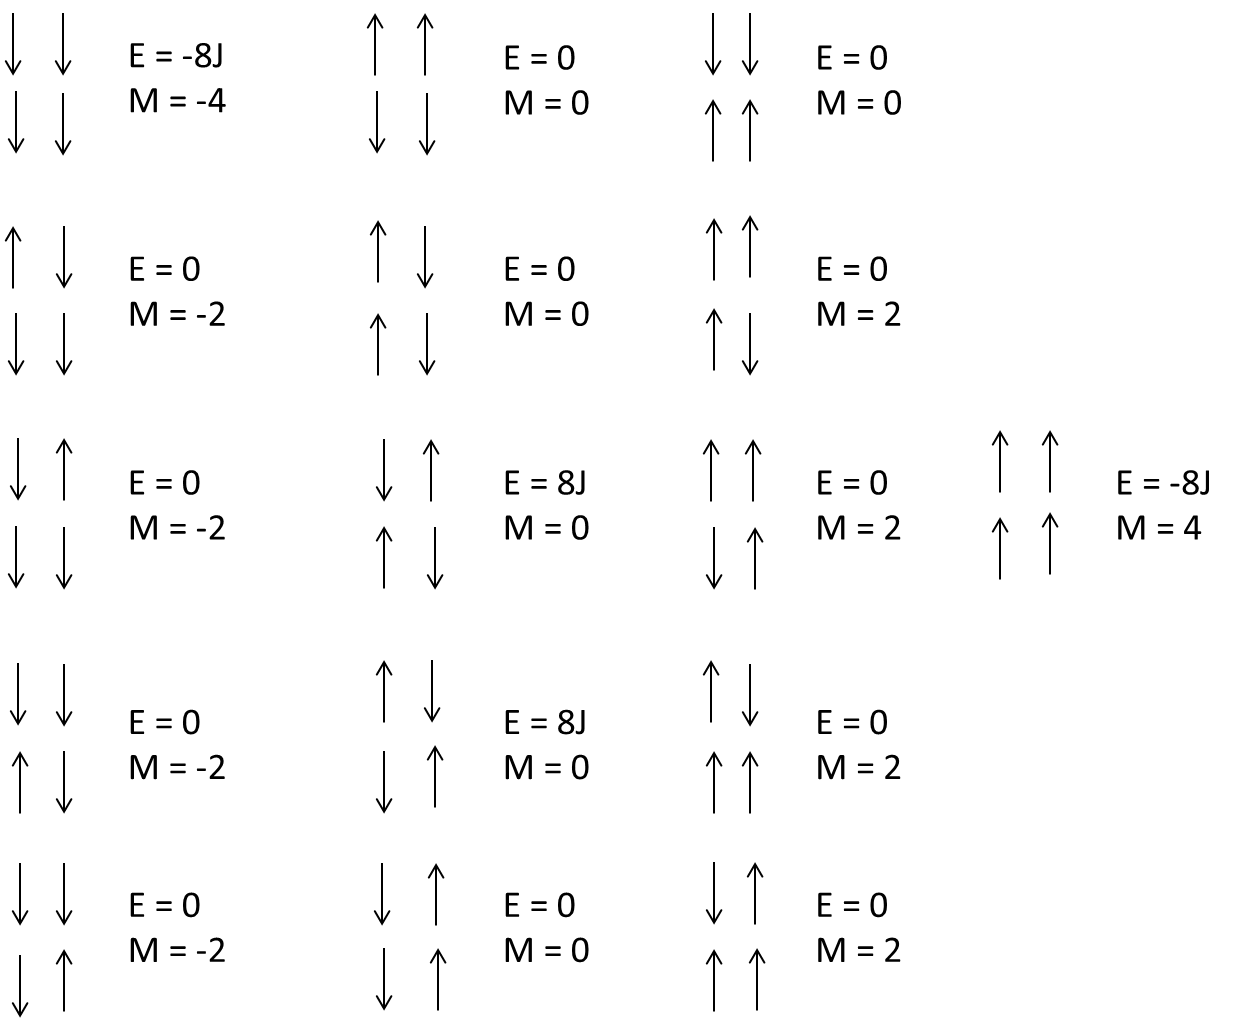
\includegraphics[width=0.6\linewidth]{../Report/spin_orientations}
}
\label{fig:spins2x2}
\end{center}
\end{figure}
\end{frame}

\begin{frame}{A $2\times2$ Lattice}
\begin{itemize}
\item Partition function:
\begin{equation}
\label{eq:partition2x2}
Z=2e^{-\frac{8J}{k_{B}T}}+2e^{\frac{8J}{k_{B}T}}+12 = 4\cosh{\frac{8J}{k_{B}T}}+12.
\end{equation}
\item Expected value of energy:
\begin{equation}
\label{eq:expe2x2}
\left<E\right> = \frac{1}{Z}\left(16Je^{-\frac{8J}{k_{B}T}}-16Je^{\frac{8J}{k_{B}T}}\right) = \frac{-32J\sinh{\frac{8J}{k_{B}T}}}{Z}.
\end{equation}
\item Magnetization and expected magnetization:
\begin{equation}
\label{eq:mag}
M_{i}=\sum_{i=1}^{N}s_{i} \Rightarrow \left<M\right>=0.
\end{equation}
\item Expected squared magnetization:
\begin{equation}
\label{eq:expabsm2x2}
\left<\left|M\right|\right> = \frac{1}{Z}\left(8e^{\frac{8J}{k_{B}T}}+4\right).
\end{equation}
\end{itemize}
\end{frame}

\begin{frame}{A $2\times2$ Lattice}
\begin{itemize}
\item Specific heat (variance of the energy of the system multiplied by some constant):
\begin{align}
\label{eq:cvdef}
C_{V} &= \frac{1}{k_{B}T^{2}}\left(\left<E^{2}\right>-\left<E\right>^{2}\right) \\ \nonumber
& = \frac{1}{k_{B}T^{2}}\left(\frac{256J^{2}\cosh{\frac{8J}{k_{B}T}}}{Z}-\left(\frac{-32J\sinh{\frac{8J}{k_{B}T}}}{Z}\right)^{2}\right) \\ \nonumber 
& =\frac{256J^{2}}{k_{B}T^{2}Z}\left(\cosh{\frac{8J}{k_{B}T}}-4\sinh^{2}{\frac{8J}{k_{B}T}}\right)
\end{align}
\end{itemize}
\end{frame}

\begin{frame}{A $2\times2$ Lattice}
\begin{itemize}
\item Magnetic susceptibility (variance of the magnetization of the system multiplied by some constant):
\begin{equation}
\label{eq:chidef}
\chi = \frac{1}{k_{B}T}\left(\left<M^{2}\right>-\left<M\right>^{2}\right) = \frac{32e^{\frac{8J}{k_{B}T}}+8}{Zk_{B}T}
\end{equation}
\end{itemize}
\end{frame}

\section{The Algorithm}

\begin{frame}{\texttt{lattice} Class}
\begin{itemize}
%\item Directly computes various statistical mechanical quantities for a lattice of a given size and temperature.  
\item Each \texttt{lattice} object has the following objects:
\begin{itemize}
\item \texttt{size}, an \texttt{int} which gives the size of the square lattice (ie. $n$ for an $n\times n$ lattice),
\item \texttt{spins}, a dynamically allocated matrix of the spins in the matrix,
\item \texttt{temp}, a \texttt{double} which gives the temperature of the matrix,
\item \texttt{averages}, a dynamically allocated vector of the averages of $E$, $E^{2}$, $M$, $M^{2}$, and $|M|$,
\item \texttt{MCcycles}, an \texttt{int} which gives the number of Monte Carlo (MC) cycles to be used in the calculation,
\item \texttt{CV}, a \texttt{double} of the specific heat,
\item \texttt{chi}, a \texttt{double} of the susceptibility,
\item \texttt{chi\_absm}, a \texttt{double} of the susceptibility calculated from $<|M|>$ rather than $<M>$ (that is, $\chi_{|M|}=<M^{2}>-<|M|>^{2}$),
\item \texttt{accepted}, an \texttt{int} of the number of Monte Carlo events accepted in the calculation, and
\item \texttt{e\_probs}, a \texttt{map} of an energy value to the number of times that energy appears in the calculations.
\end{itemize}
\end{itemize}
\end{frame}

\begin{frame}{\texttt{lattice} Class}
\begin{itemize}
\item In addition to a default constructor, copy constructor, and  destructor, \texttt{lattice} has a:
\begin{itemize}
\item constructor from a size, temperature, number of Monte Carlo cycles, and the option to start at a lowest-energy state,
\item several "get" functions (eg. \texttt{get\_{E}()}), which returns some statistical mechanical quantities,
\item several "set" function (eg. \texttt{set\_temp(double t)}), which resets and recalculates some variable,
\item \texttt{plot\_eprobs(string name)}, which plots the probability of various energy values $E$ appearing in the calculations, and
\item \texttt{calc\_stat\_quants()}, which is a private function which performs all of the calculations and sets all of the variables as the \texttt{lattice} object is constructed.
\end{itemize} 
\end{itemize}
\end{frame}

\begin{frame}{\texttt{calc\_stat\_quants()} and Monte Carlo}
\begin{itemize}
\item Monte Carlo is required in any computer simulation of the Ising model.
\item This is implemented in the \texttt{calc\_stat\_quants()} function, which is called by all constructors after a random (or not) initial state is set for the lattice:
\begin{enumerate}
\item Calculating the initial energy with periodic boundary conditions
\item Monte Carlo simulation (Metropolis Algorithm)
\item Update statistical mechanical quantities 
\end{enumerate}
\end{itemize}
\end{frame}

\begin{frame}{Metropolis Algorithm}
\begin{enumerate}
\item Iterate through integers \texttt{cycle} which are less than the \texttt{MCcycles} parameter
\item Randomly change one of the spins in the lattice 
\item Calculate the change in energy resulting from changing this spin by calling the \texttt{nearest\_neighbors()} function  
\item If change in energy is negative, generate a random number \texttt{myrand} (in $\left[0,1\right]$) and compare to $w=e^{-\frac{\Delta E}{k_{B}T}}$
\begin{itemize}
\item $w \leq$ \texttt{myrand}: keep the change in spin
\item $w >$ \texttt{myrand}: keep the spin matrix as it was before.
\end{itemize}
\end{enumerate}
\end{frame}

\begin{frame}{Possible Values of $\Delta E$ for a $2\times2$ Lattice}
\begin{figure}[ht]
\begin{center}
\subfigure[]{
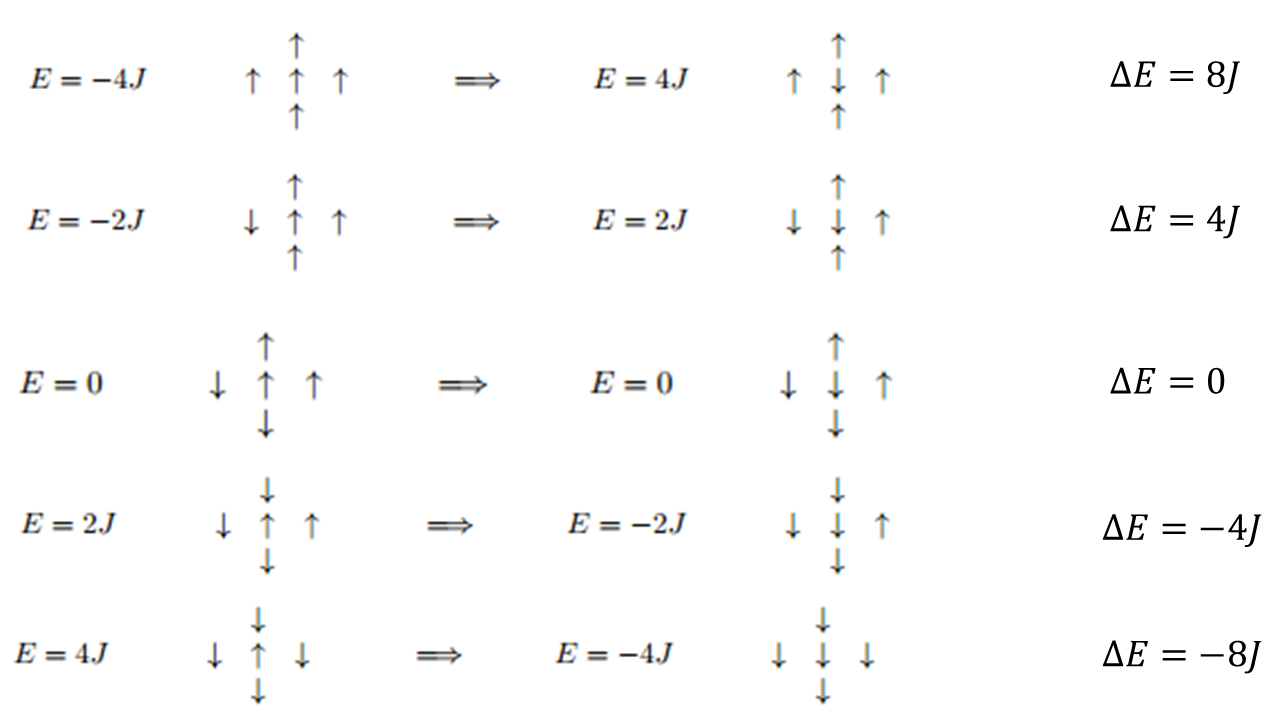
\includegraphics[width=0.6\textwidth]{../Report/deltaEs}
}
\caption{The possible values of $\Delta E$ for the $2\times2$ lattice after changing one spin~\cite{lecture}.}
\label{fig:deltaEs}
\end{center}
\end{figure}
\end{frame}

\section{Benchmarks}

\begin{frame}{Expected Results for $2\times2$ Lattice}
\begin{table}[ht]
\begin{center}
\begin{tabular}{c|c} \hline
Statistical Quantity & $2\times2$ Accepted Value \\ \hline
$Z$ & 5973.917 \\
$\left<E\right>$ &  -7.984 \\
$\left<\left|M\right|\right>$ & 3.993 \\
$\left<E^{2}\right>$ & 63.871 \\
$\left<M^{2}\right>$ & 15.969 \\
$C_{V}$ & 0.127 \\
$\chi$ & 16.001
\end{tabular}
\caption{The accepted calculated values for the $2\times2$ lattice under the Ising model for a temperature $T=1/k_{B}$.}
\label{tab:2x2exp}
\end{center}
\end{table}
\end{frame}

\begin{frame}{Computed Values for $2\times2$ Lattice}
\vspace{-0.4cm}
\begin{figure}[ht]
\begin{center}
\subfigure[]{
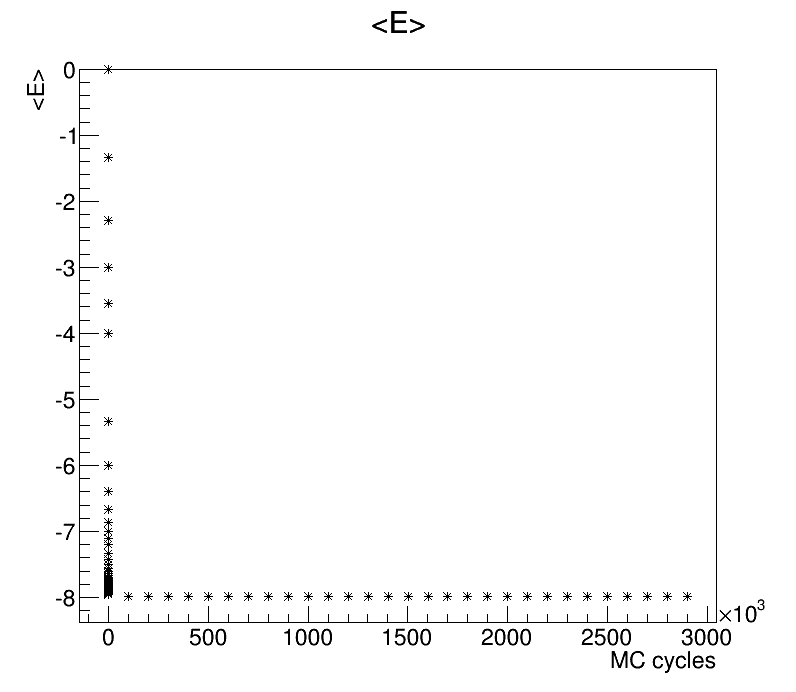
\includegraphics[width=0.27\textwidth]{../Report/benchmarks/plots/plots_random_meanE_size2_temp1}
}
\subfigure[]{
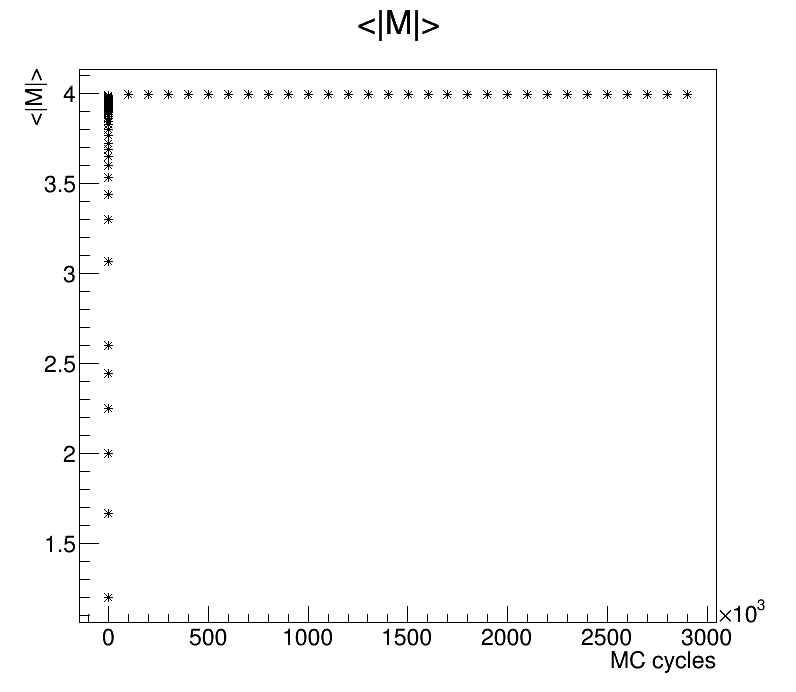
\includegraphics[width=0.27\textwidth]{../Report/benchmarks/plots/plots_random_meanAbsM_size2_temp1}
} \\
\subfigure[]{
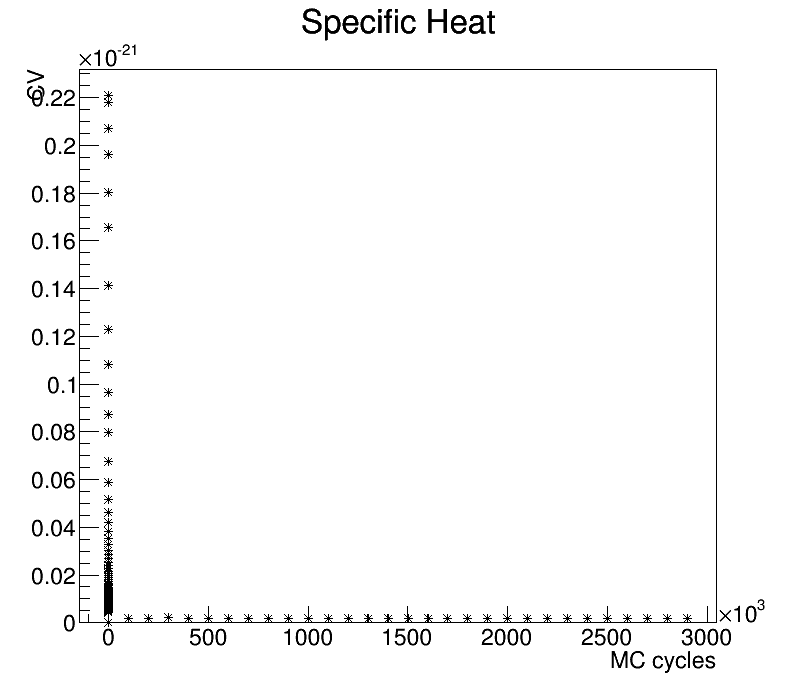
\includegraphics[width=0.27\textwidth]{../Report/benchmarks/plots/plots_random_CV_size2_temp1}
}
\subfigure[]{
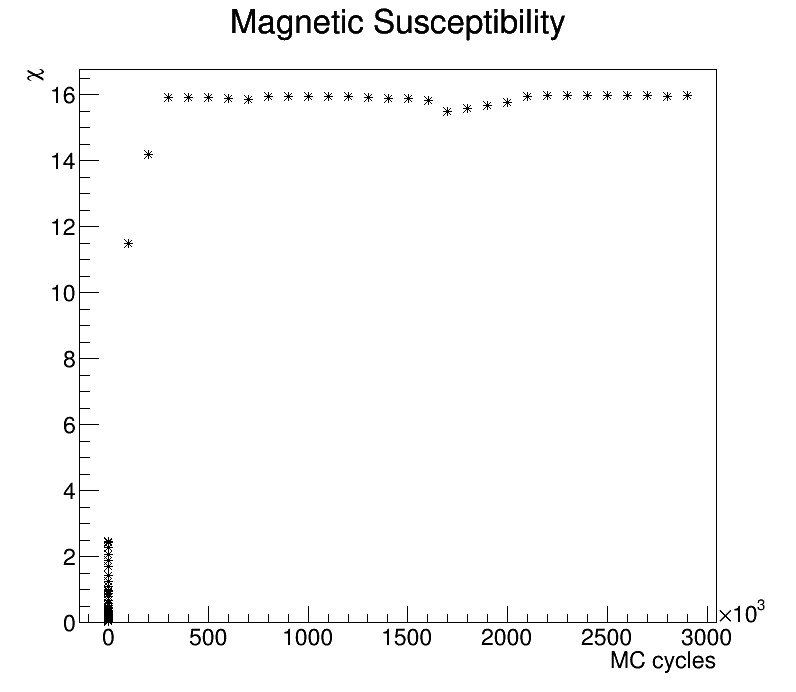
\includegraphics[width=0.27\textwidth]{../Report/benchmarks/plots/plots_random_chi_size2_temp1}
}\vspace{-0.4cm}
\caption{The (a) $<E>$, (b) $<|M|>$, (c) $C_{V}$, and (d) $\chi$ for a $2\times2$ lattice at temperature $T=1/k_{B}$.}
\label{fig:benchmarks}
\end{center}
\end{figure}
\end{frame}

\section{Results}

\begin{frame}{Number of Required Monte Carlo}
\vspace{-0.4cm}
\begin{figure}[h]
\begin{center}
\subfigure[]{
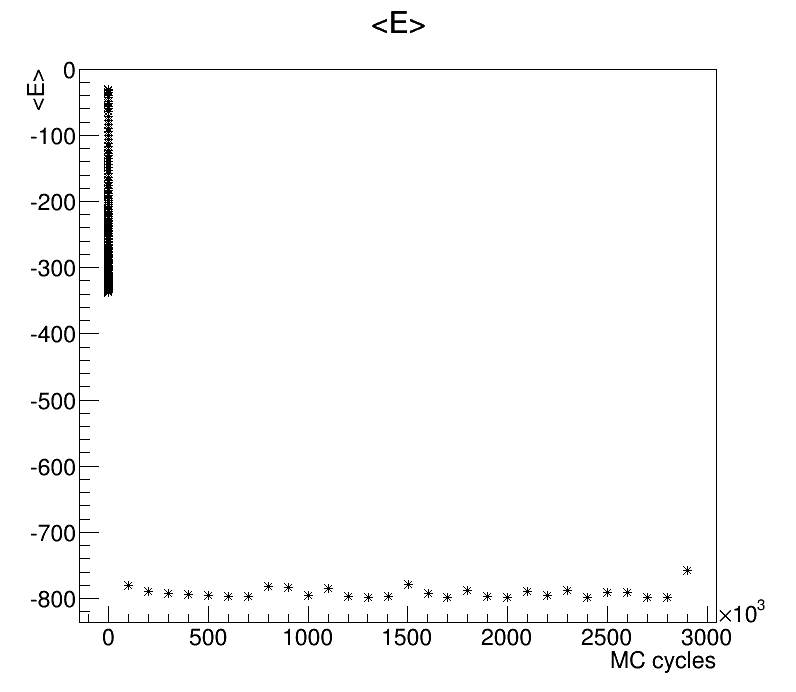
\includegraphics[width=0.27\textwidth]{../Report/plots/partcandd/plots_random_meanE_size20_temp1}
}
\subfigure[]{
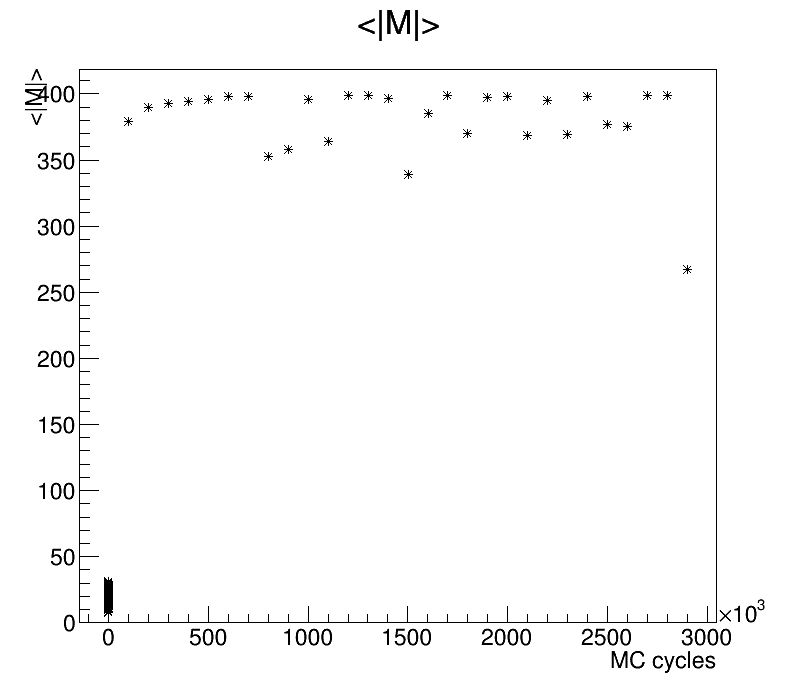
\includegraphics[width=0.27\textwidth]{../Report/plots/partcandd/plots_random_meanAbsM_size20_temp1}
} \\
\subfigure[]{
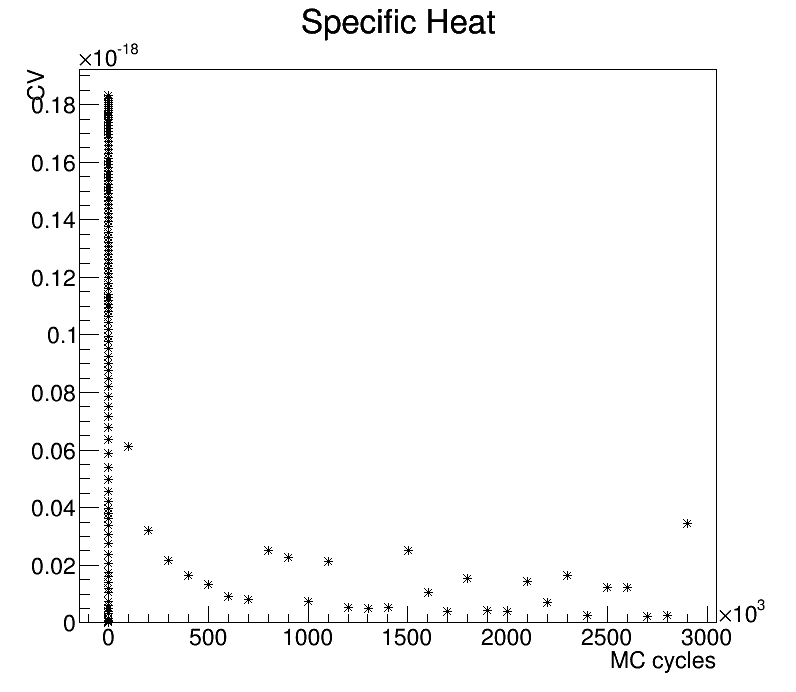
\includegraphics[width=0.27\textwidth]{../Report/plots/partcandd/plots_random_CV_size20_temp1}
}
\subfigure[]{
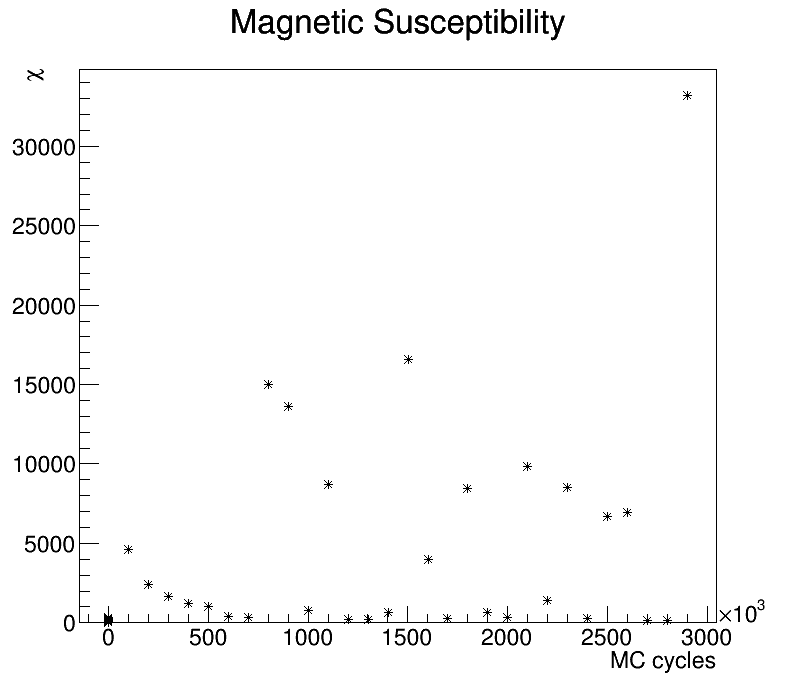
\includegraphics[width=0.27\textwidth]{../Report/plots/partcandd/plots_random_chi_size20_temp1}
}\vspace{-0.4cm}
\caption{Statistical quantities for a $20\times20$ lattice at a temperature $T=1/k_{B}$ with an initial state of a random selection of spins.}
\label{fig:size20temp1rando}
\end{center}
\end{figure}
\end{frame}

\begin{frame}{Number of Required Monte Carlo}
\vspace{-0.4cm}
\begin{figure}[h]
\begin{center}
\subfigure[]{
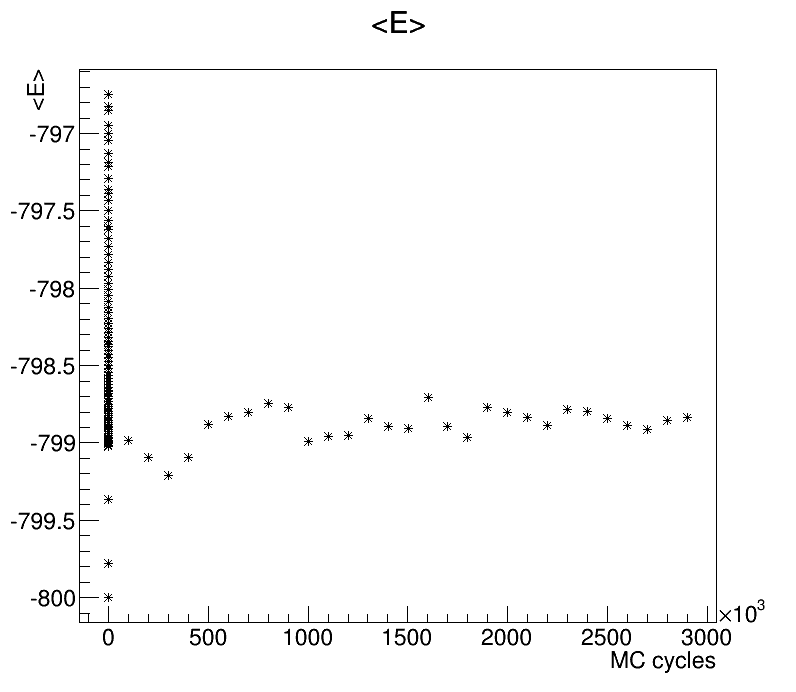
\includegraphics[width=0.27\textwidth]{../Report/plots/partcandd/plots_steady_meanE_size20_temp1}
}
\subfigure[]{
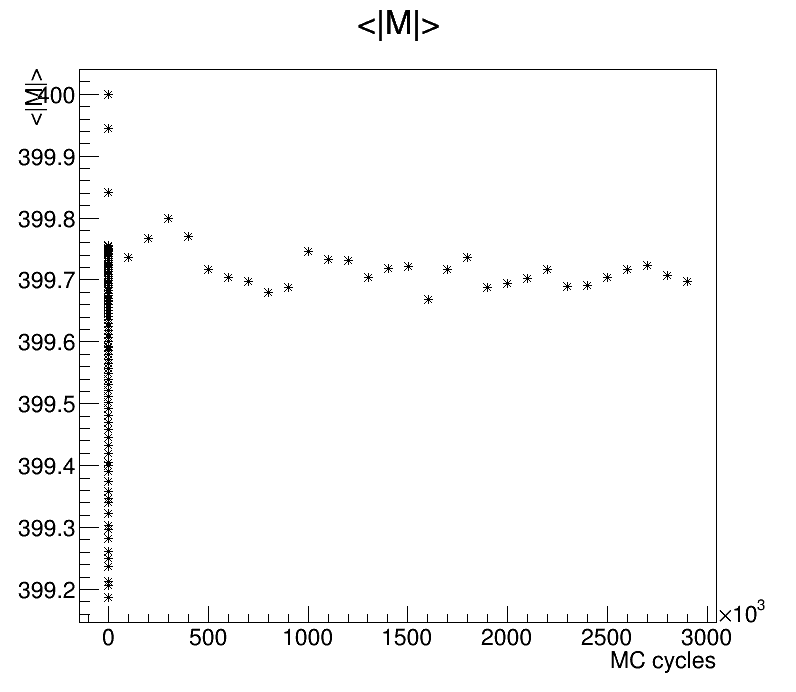
\includegraphics[width=0.27\textwidth]{../Report/plots/partcandd/plots_steady_meanAbsM_size20_temp1}
} \\
\subfigure[]{
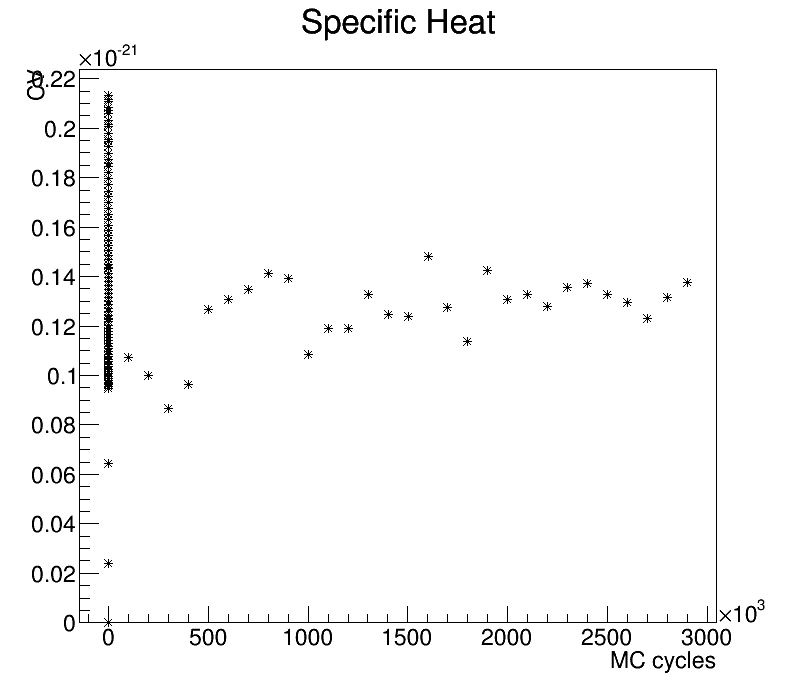
\includegraphics[width=0.27\textwidth]{../Report/plots/partcandd/plots_steady_CV_size20_temp1}
}
\subfigure[]{
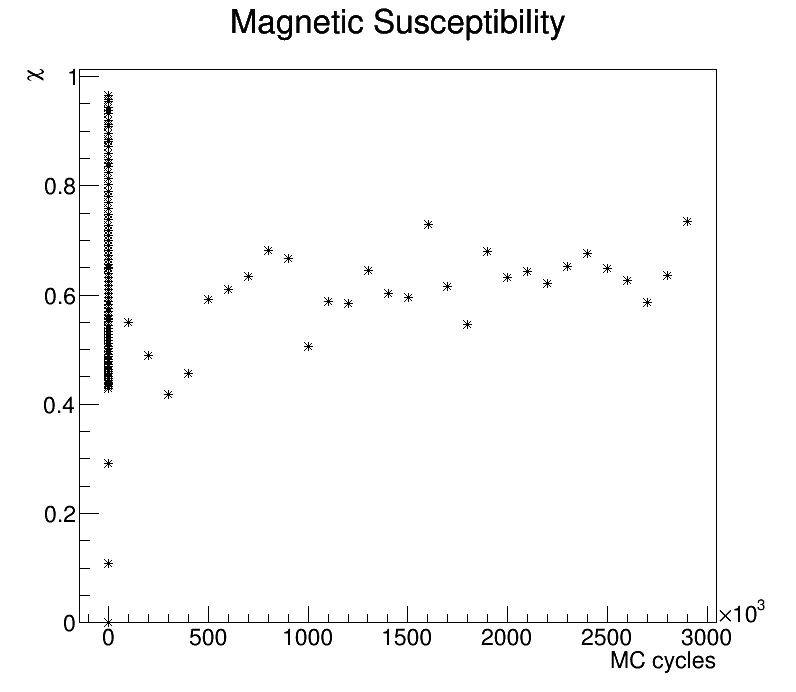
\includegraphics[width=0.27\textwidth]{../Report/plots/partcandd/plots_steady_chi_size20_temp1}
}\vspace{-0.4cm}
\caption{Statistical quantities for a $20\times20$ lattice at a temperature $T=1/k_{B}$ with a steady-state initial state.}
\label{fig:size20temp1steady}
\end{center}
\end{figure}
\end{frame}

\begin{frame}{Temperature Dependence of MC}
\vspace{-0.4cm}
\begin{figure}[h]
\begin{center}
\subfigure[]{
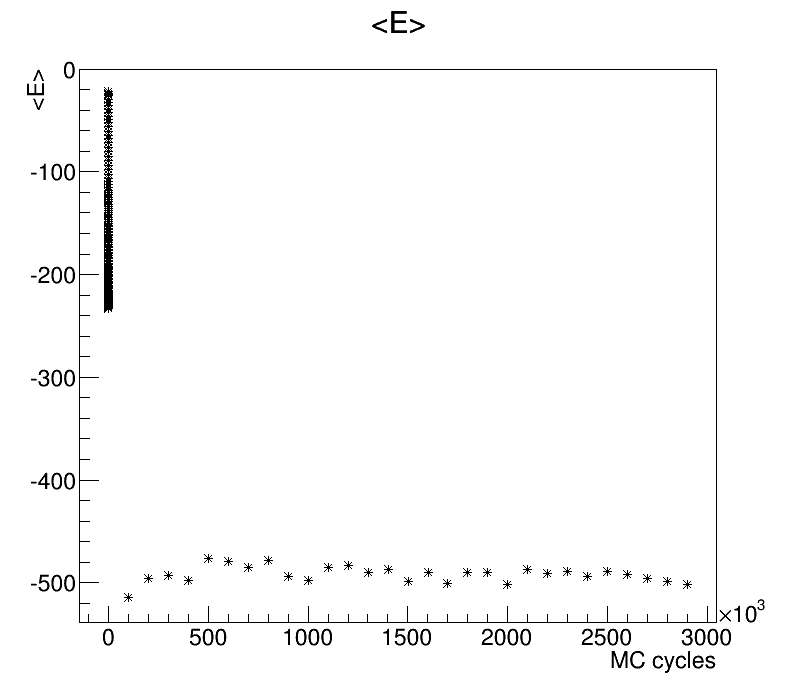
\includegraphics[width=0.27\textwidth]{../Report/plots/partcandd/plots_random_meanE_size20_temp24}
}
\subfigure[]{
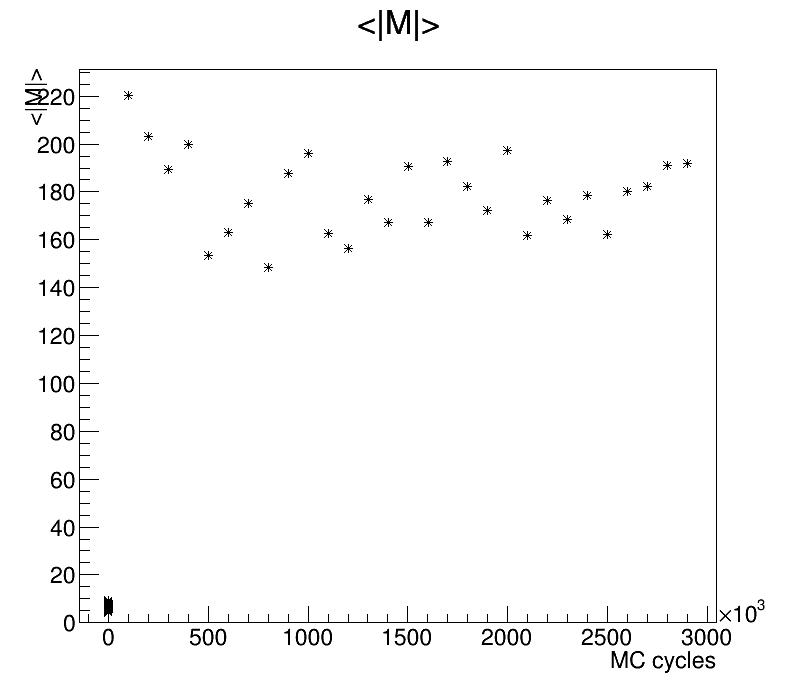
\includegraphics[width=0.27\textwidth]{../Report/plots/partcandd/plots_random_meanAbsM_size20_temp24}
} \\
\subfigure[]{
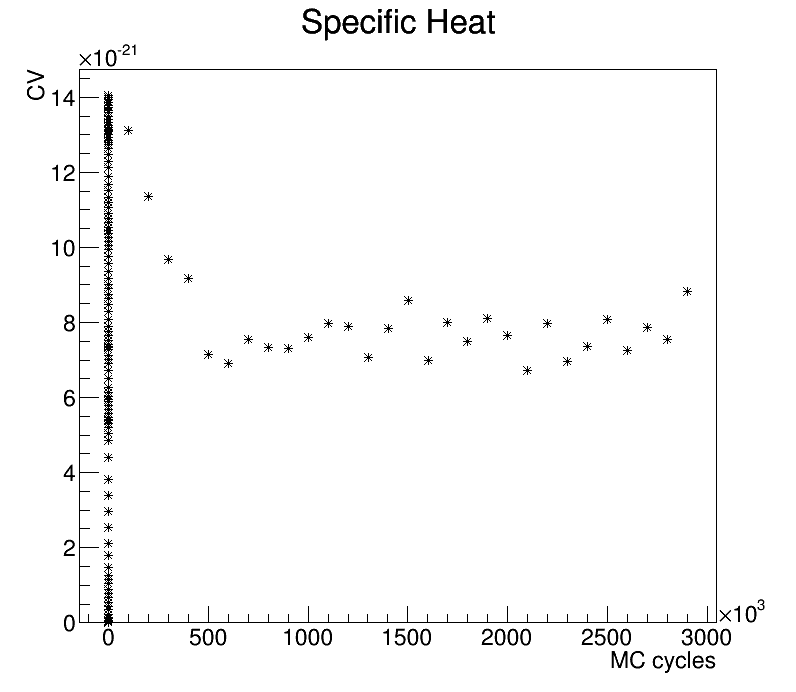
\includegraphics[width=0.27\textwidth]{../Report/plots/partcandd/plots_random_CV_size20_temp24}
}
\subfigure[]{
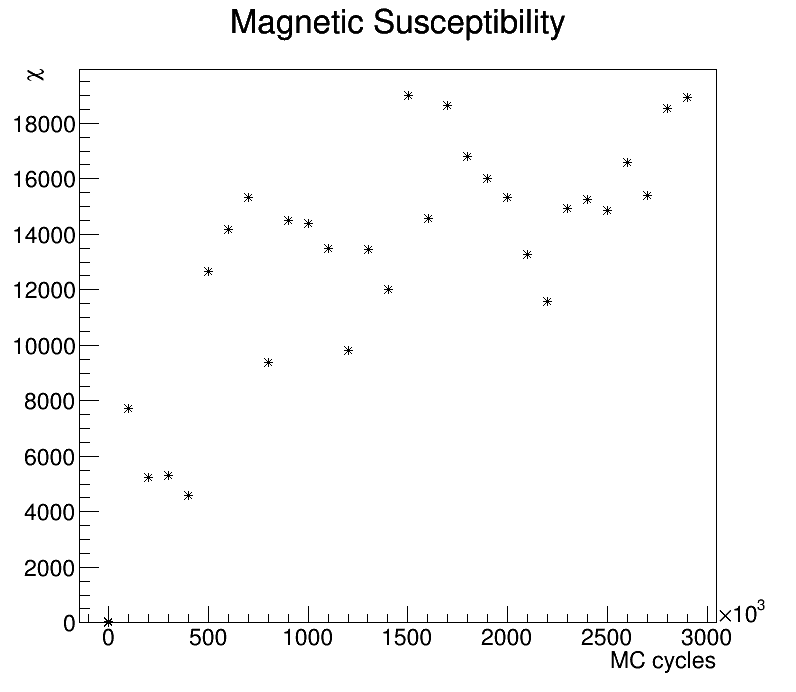
\includegraphics[width=0.27\textwidth]{../Report/plots/partcandd/plots_random_chi_size20_temp24}
}\vspace{-0.4cm}
\caption{Statistical quantities for a $20\times20$ lattice at a temperature $T=2.4/k_{B}$ with an initial state of a random selection of spins.}
\label{fig:size20temp24rando}
\end{center}
\end{figure}
 \end{frame}

\begin{frame}{Temperature Dependence of MC}
\vspace{-0.4cm}
\begin{figure}[h]
\begin{center}
\subfigure[]{
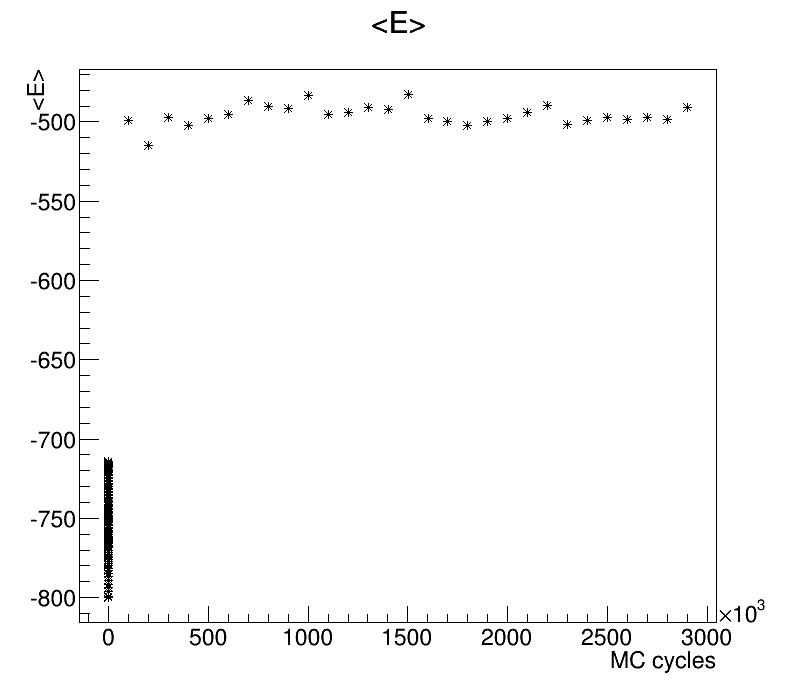
\includegraphics[width=0.27\textwidth]{../Report/plots/partcandd/plots_steady_meanE_size20_temp24}
}
\subfigure[]{
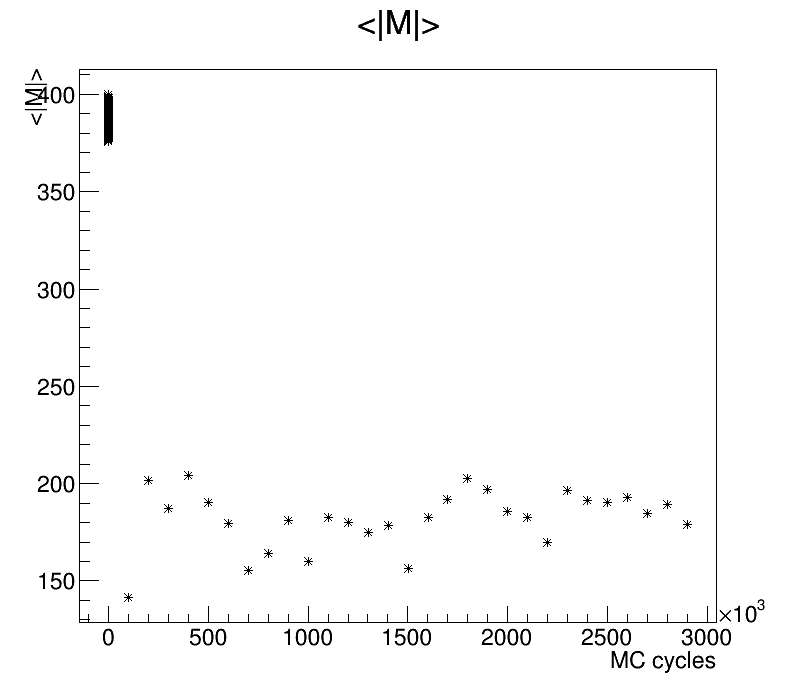
\includegraphics[width=0.27\textwidth]{../Report/plots/partcandd/plots_steady_meanAbsM_size20_temp24}
} \\
\subfigure[]{
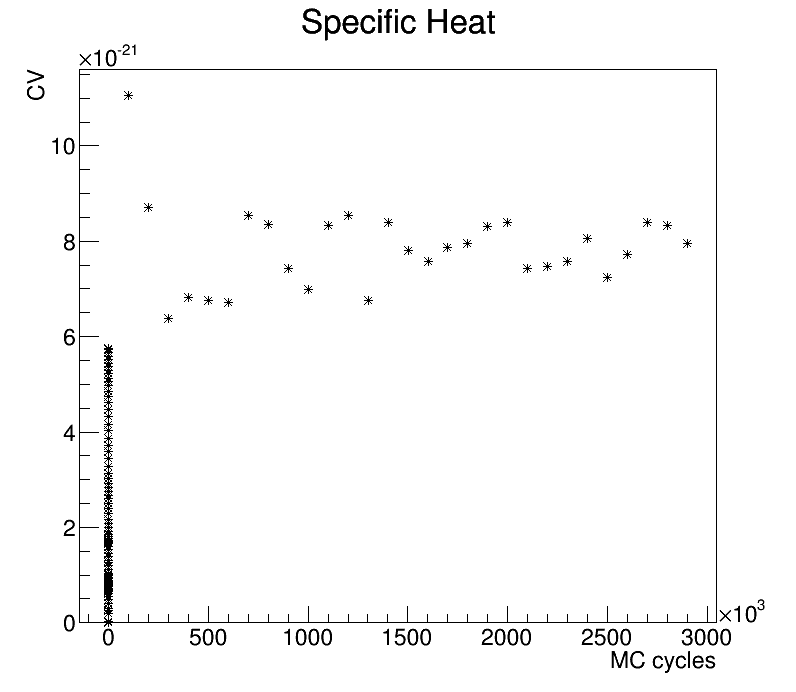
\includegraphics[width=0.27\textwidth]{../Report/plots/partcandd/plots_steady_CV_size20_temp24}
}
\subfigure[]{
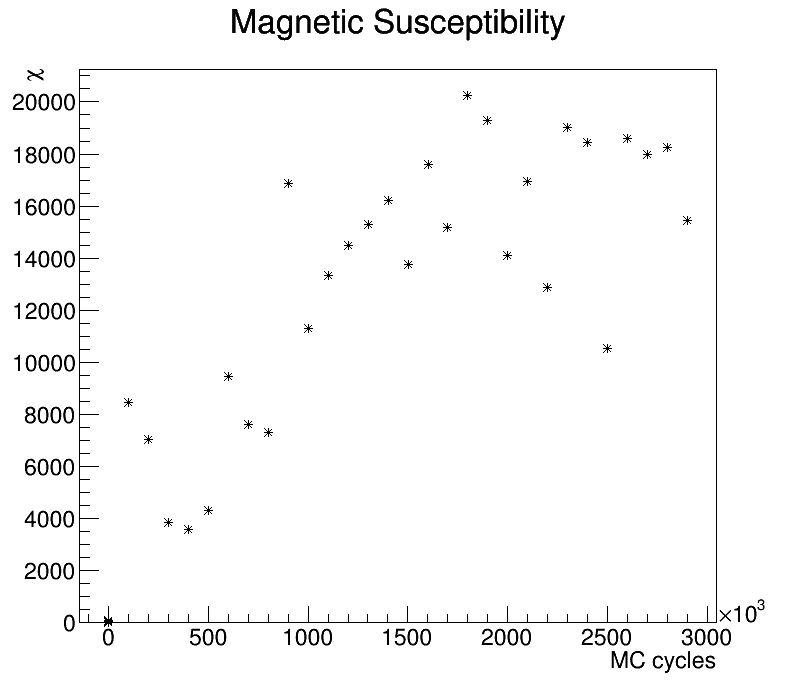
\includegraphics[width=0.27\textwidth]{../Report/plots/partcandd/plots_steady_chi_size20_temp24}
}\vspace{-0.4cm}
\caption{Statistical quantities for a $20\times20$ lattice at a temperature $T=2.4/k_{B}$ with a steady-state initial state.}
\label{fig:size20temp24steady}
\end{center}
\end{figure}
\end{frame}

\begin{frame}{$P\left(E\right)$}
\begin{itemize}
\item $P(E)$: number of times a given energy $E$ occurs in the MC process divided by the number of cycles used. 
\end{itemize}

\begin{figure}[h]
\begin{center}
\subfigure[]{
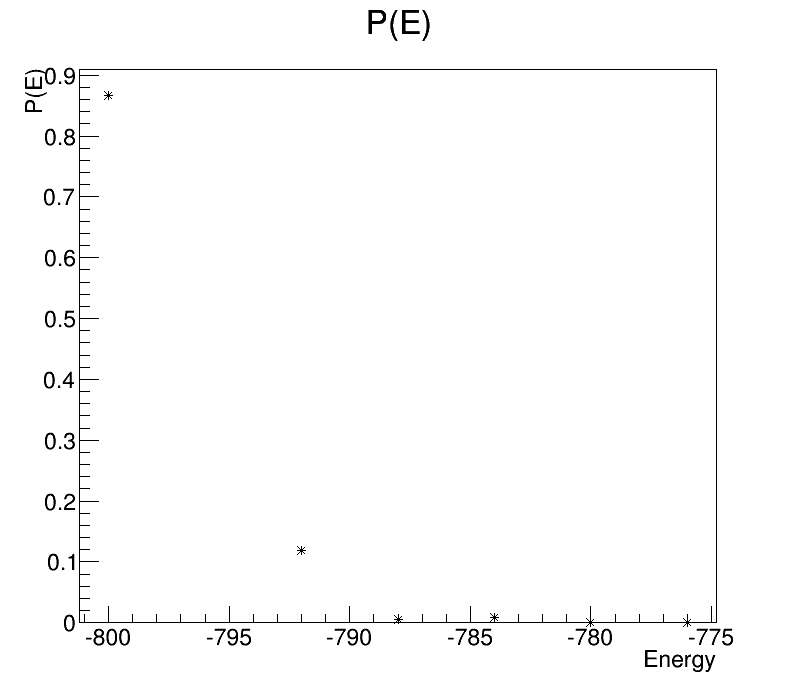
\includegraphics[width=0.27\textwidth]{../Report/plots/partcandd/plots_steady_pofE_size20_temp1}
}
\subfigure[]{
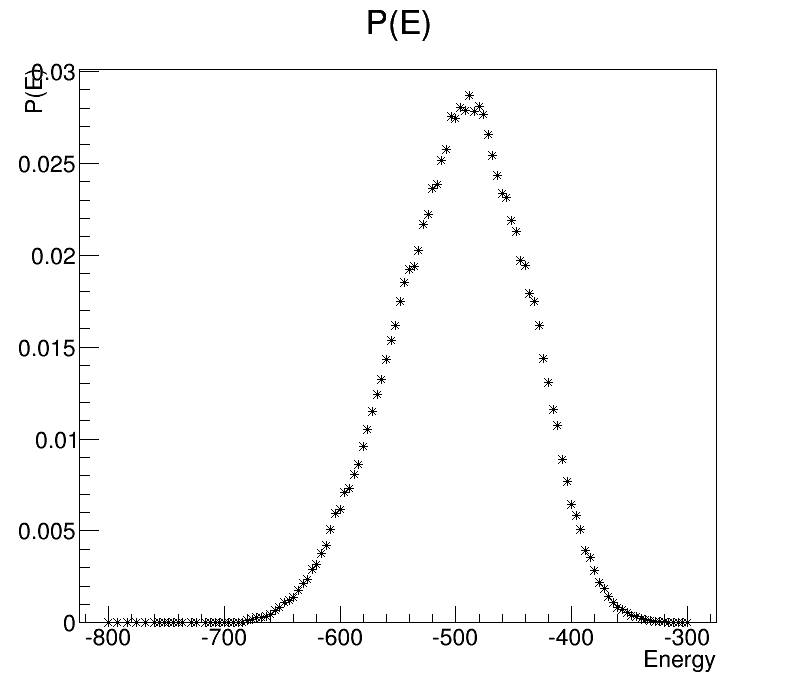
\includegraphics[width=0.27\textwidth]{../Report/plots/partcandd/plots_steady_pofE_size20_temp24}
} 
\caption{$P(E)$ for a $20\times20$ lattice at a temperature of (a) $T=1/k_{B}$ and (b) $T=2.4/k_{B}$.}
\label{fig:size20pofE}
\end{center}
\end{figure}
\end{frame}

\begin{frame}{Critical Temperature}
\begin{itemize}
\item Phase transition: when the matter undergoes a change of phase (eg. liquid to gas or solid to liquid, etc.)
\begin{itemize}
\item Occurs at the critical temperature of the system, denoted $T_{C}$
\end{itemize}
\item Near $T_{C}$, many physical quantities can be characterized by a power law exponent.  
\begin{itemize}
\item Mean magnetization:
\begin{equation}
\label{eq:tcmag}
<M(T)>\sim(T-T_{C})^{1/8},
\end{equation}
\item Heat capacity:
\begin{equation}
\label{eq:tccv}
C_{V}(T)\sim|T_{C}-T|^{0},
\end{equation}
\item Susceptibility:
\begin{equation}
\label{eq:tcchi}
\chi(T)\sim|T-T_{C}|^{\frac{7}{4}}.
\end{equation}
\item Correlation length $\xi$ (measure of how correlated the spins within the lattice are to one another)~\cite{lecture}: 
\begin{equation}
\label{eq:tccorr}
\xi(T)\sim|T_{C}-T|^{-\nu}
\end{equation}
\end{itemize}
\end{itemize}
\end{frame}

\begin{frame}{Critical Temperature of an Infinite Lattice}
\begin{itemize}
\item $\xi$ scales with the size of the lattice, so we can use a finite lattice to approximate an infinite system
\begin{equation}
\label{eq:tcscale}
T_{C}(L)-T_{C}(L=\infty)=aL^{\frac{1}{\nu}}
\end{equation}
for some constant $a$ for a lattice of size $L$.  
\item By setting $T=T_{C}$, we can see~\cite{lecture}
\begin{align}
\label{eq:tcquants}
<M(T)> & \sim  (T-T_{C})^{\frac{1}{8}} \rightarrow  L^{\frac{1}{8\nu}} \\
C_{V}(T) & \sim  |T_{C}-T|^{-\frac{7}{4}} \rightarrow  L^{0} \\
\chi(T) & \sim  |T_{C}-T|^{0} \rightarrow L^{\frac{7}{4\nu}}. 
\end{align}
\item In order to study $T_{C}$, we look for indications of a phase transition in the graphs of $<E>$, $<|M|>$, $C_{V}$, and $\chi$\footnote{Here, $\chi$ is calculated with $<|M|>$.} for various lattice sizes.  
\end{itemize}
\end{frame}

\begin{frame}{Statistical Quantities Used to Estimate $T_{C}$}
\vspace{-0.4cm}
\begin{figure}[h]
\begin{center}
\subfigure[]{
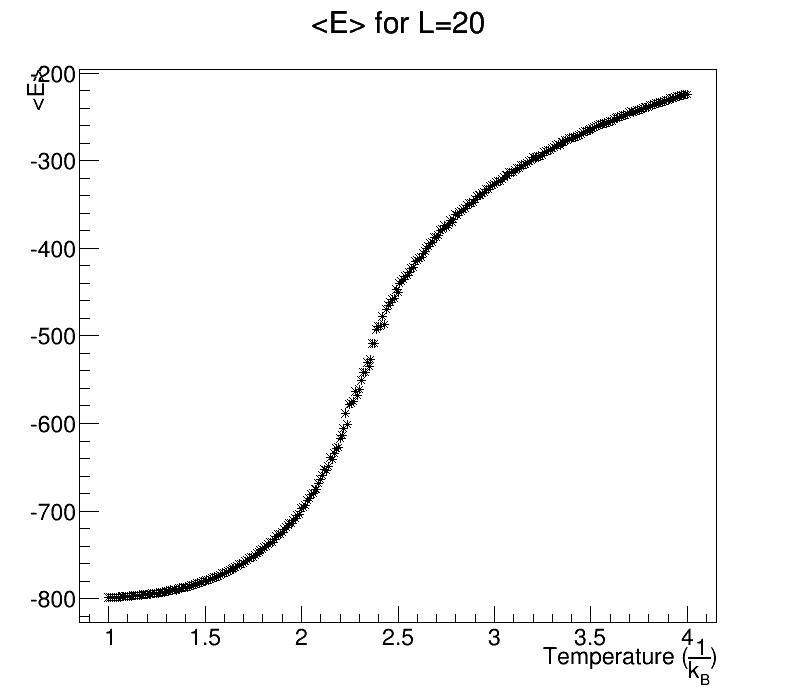
\includegraphics[width=0.27\textwidth]{../Report/plots/parte/expE_latsize20}
}
\subfigure[]{
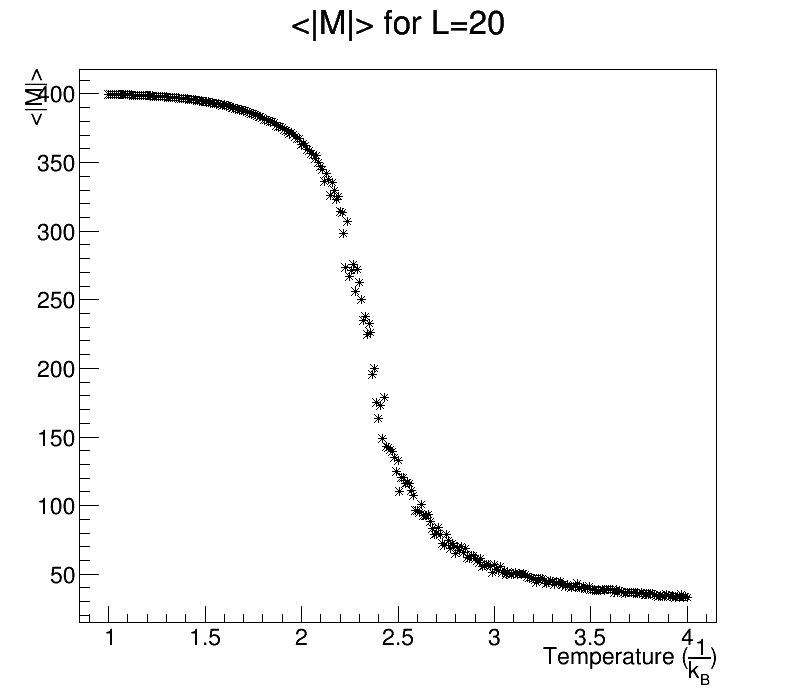
\includegraphics[width=0.27\textwidth]{../Report/plots/parte/expAbsM_latsize20}
} \\
\subfigure[]{
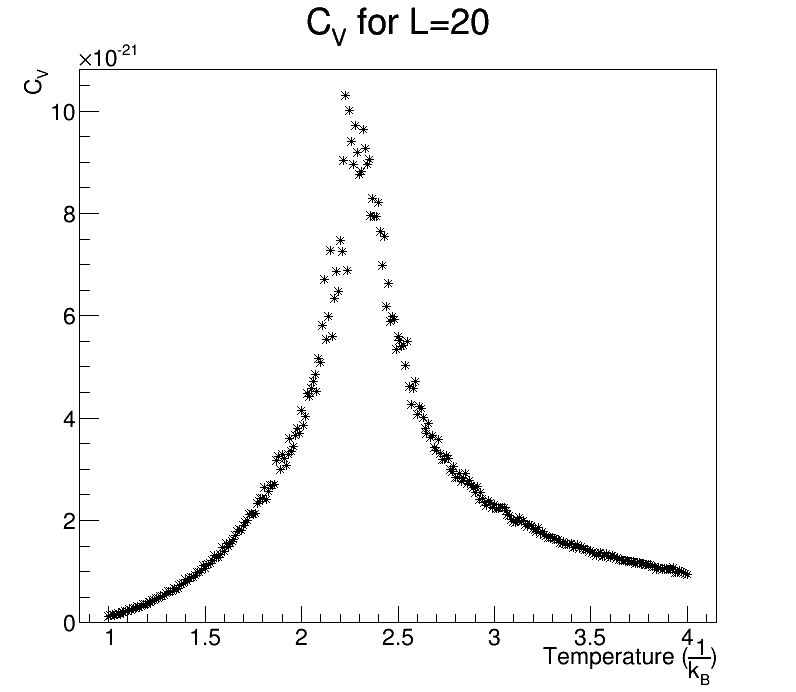
\includegraphics[width=0.27\textwidth]{../Report/plots/parte/CV_latsize20}
}
\subfigure[]{
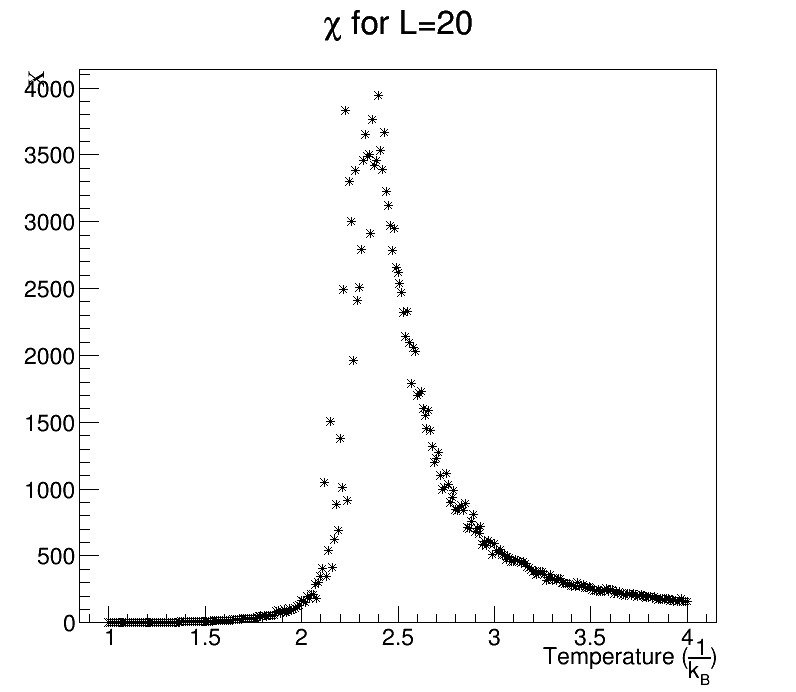
\includegraphics[width=0.27\textwidth]{../Report/plots/parte/susceptibility_latsize20}
}\vspace{-0.4cm}
\caption{Statistical quantities for a $20\times20$ lattice with a steady initial state plotted against the temperature.}
\label{fig:latsize20}
\end{center}
\end{figure}
\end{frame}

\begin{frame}{Statistical Quantities Used to Estimate $T_{C}$}
\vspace{-0.4cm}
\begin{figure}[h]
\begin{center}
\subfigure[]{
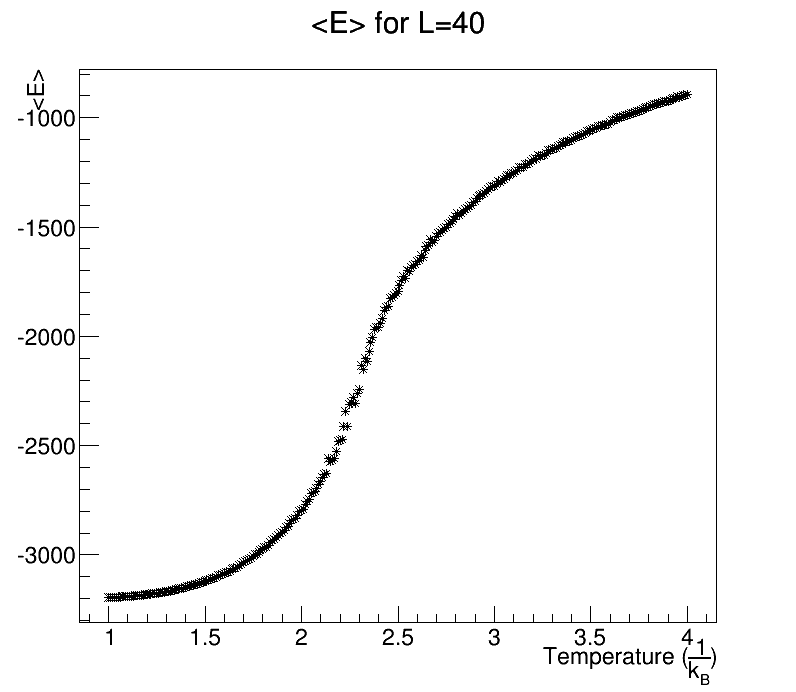
\includegraphics[width=0.27\textwidth]{../Report/plots/parte/expE_latsize40}
}
\subfigure[]{
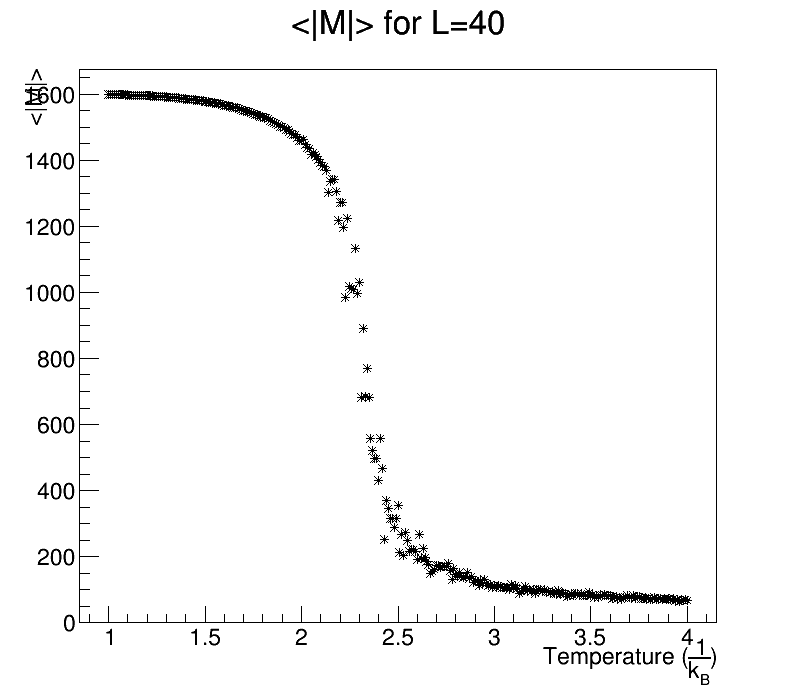
\includegraphics[width=0.27\textwidth]{../Report/plots/parte/expAbsM_latsize40}
} \\
\subfigure[]{
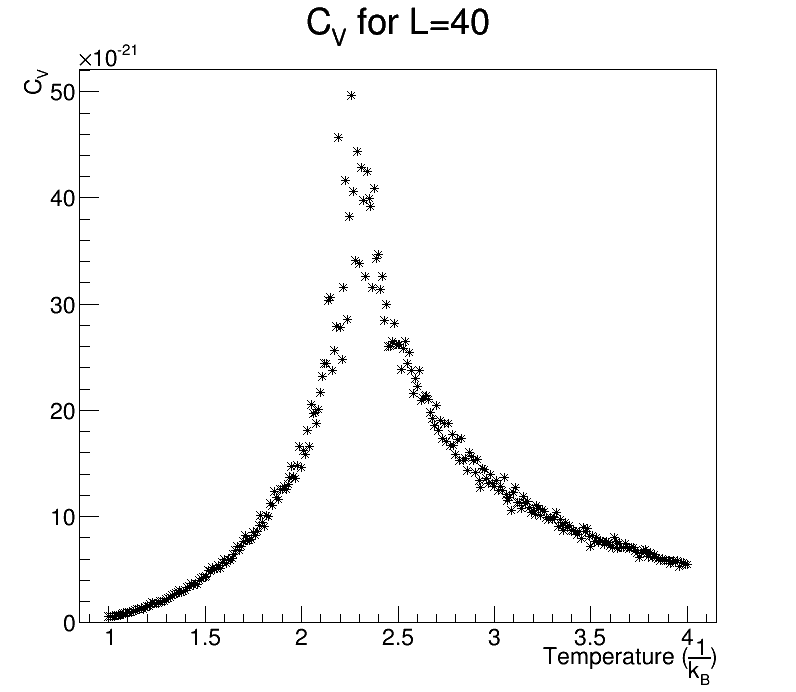
\includegraphics[width=0.27\textwidth]{../Report/plots/parte/CV_latsize40}
}
\subfigure[]{
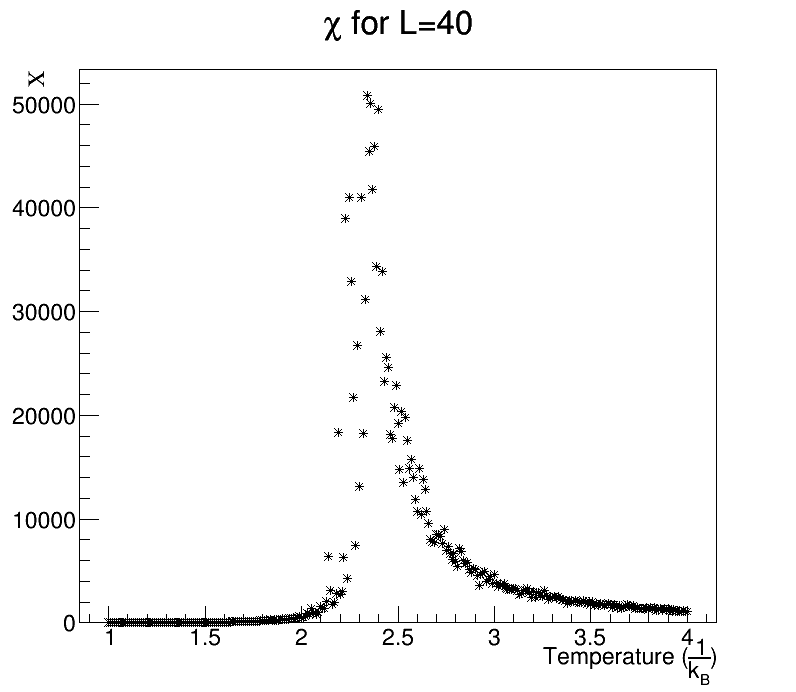
\includegraphics[width=0.27\textwidth]{../Report/plots/parte/susceptibility_latsize40}
}\vspace{-0.4cm}
\caption{Statistical quantities for a $40\times40$ lattice with a steady initial state plotted against the temperature.}
\label{fig:latsize40}
\end{center}
\end{figure}
\end{frame}

\begin{frame}{Statistical Quantities Used to Estimate $T_{C}$}
\vspace{-0.4cm}
\begin{figure}[h]
\begin{center}
\subfigure[]{
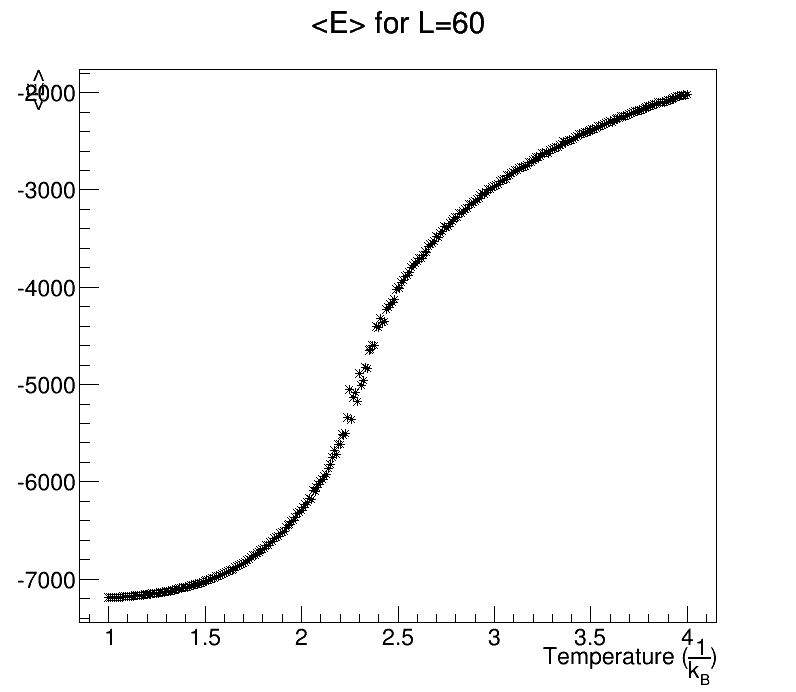
\includegraphics[width=0.27\textwidth]{../Report/plots/parte/expE_latsize60}
}
\subfigure[]{
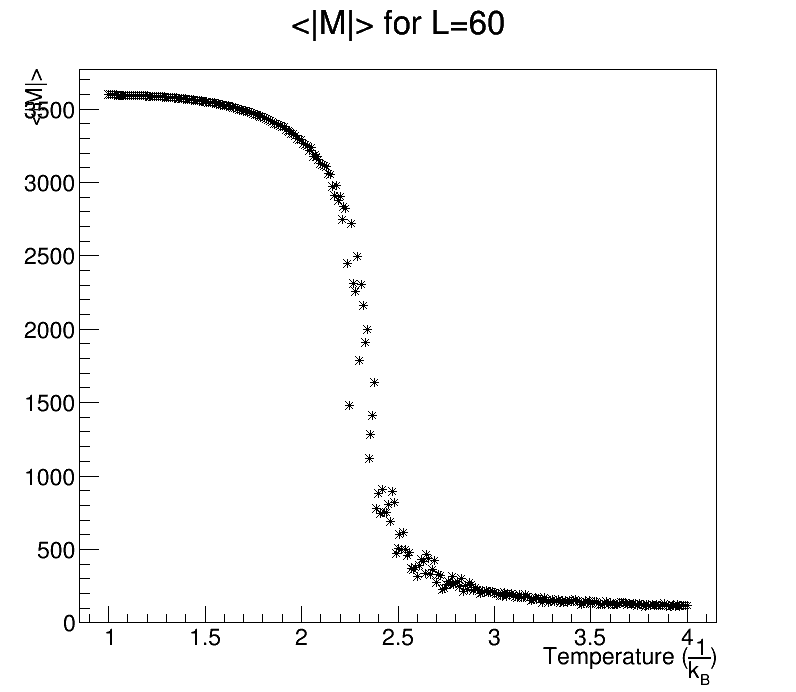
\includegraphics[width=0.27\textwidth]{../Report/plots/parte/expAbsM_latsize60}
} \\
\subfigure[]{
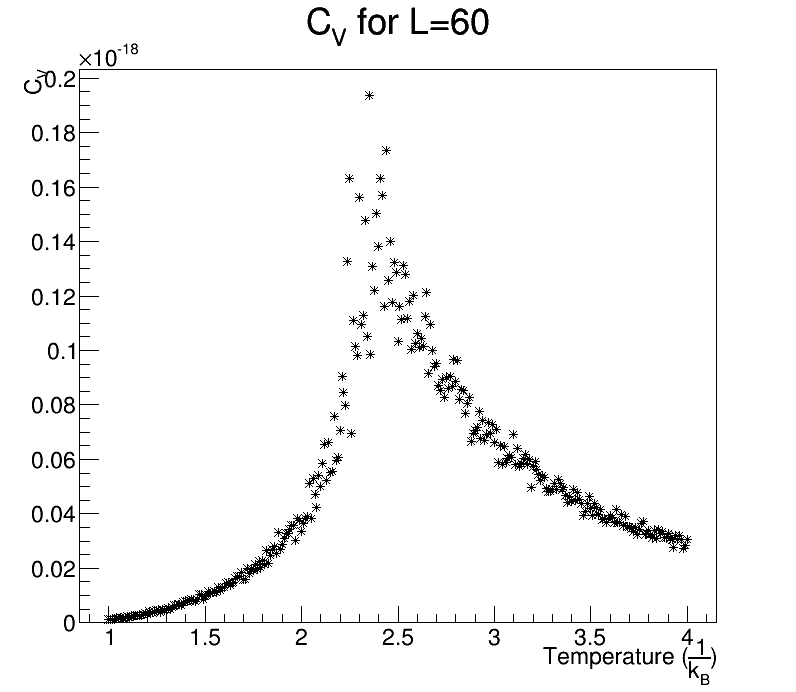
\includegraphics[width=0.27\textwidth]{../Report/plots/parte/CV_latsize60}
}
\subfigure[]{
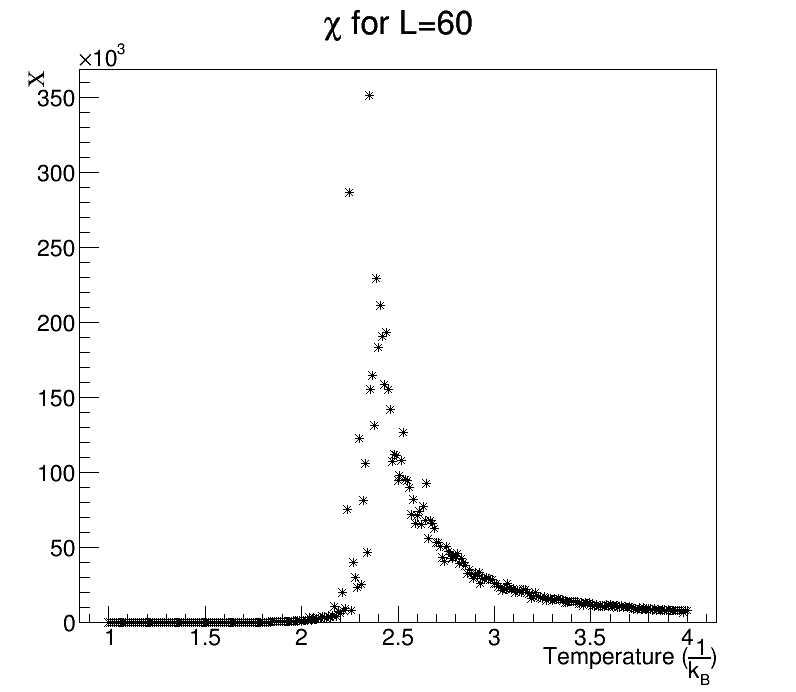
\includegraphics[width=0.27\textwidth]{../Report/plots/parte/susceptibility_latsize60}
}\vspace{-0.4cm}
\caption{Statistical quantities for a $60\times60$ lattice with a steady initial state plotted against the temperature.}
\label{fig:latsize60}
\end{center}
\end{figure}
\end{frame}

\begin{frame}{Statistical Quantities Used to Estimate $T_{C}$}
\vspace{-0.4cm}
\begin{figure}[h]
\begin{center}
\subfigure[]{
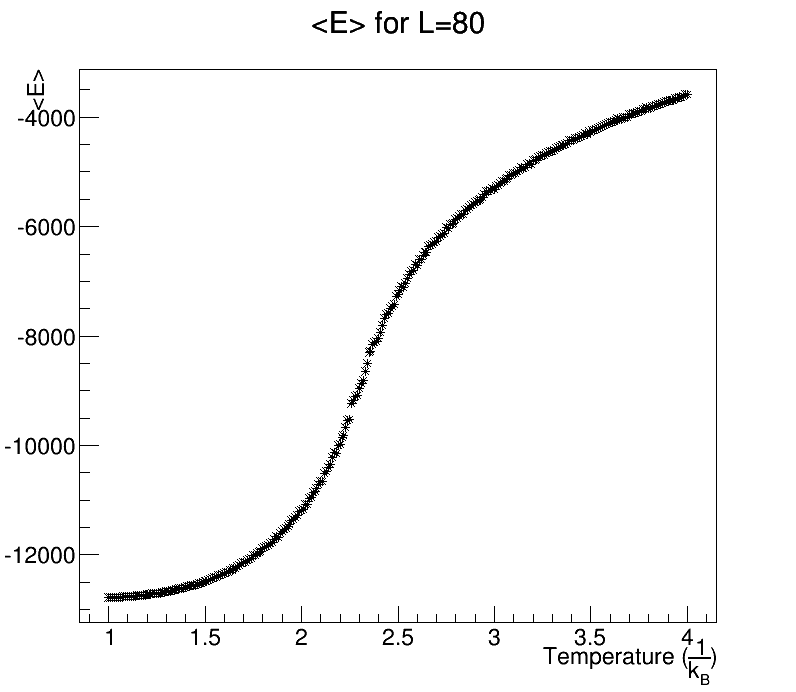
\includegraphics[width=0.27\textwidth]{../Report/plots/parte/expE_latsize80}
}
\subfigure[]{
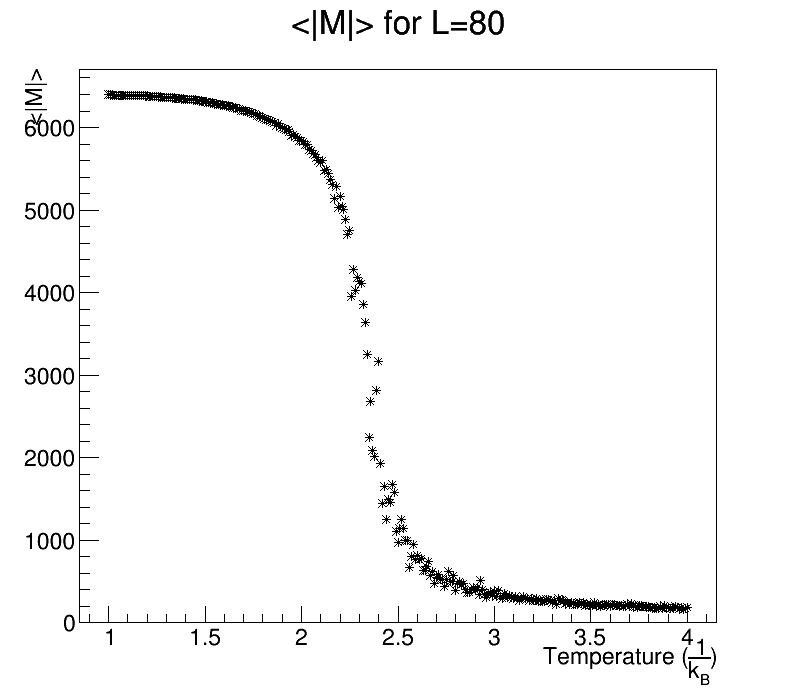
\includegraphics[width=0.27\textwidth]{../Report/plots/parte/expAbsM_latsize80}
} \\
\subfigure[]{
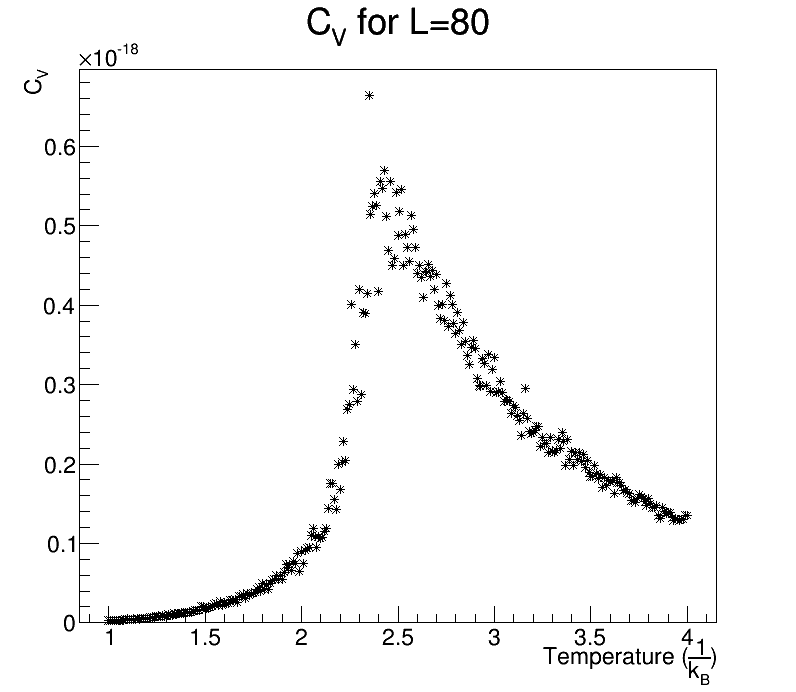
\includegraphics[width=0.27\textwidth]{../Report/plots/parte/CV_latsize80}
}
\subfigure[]{
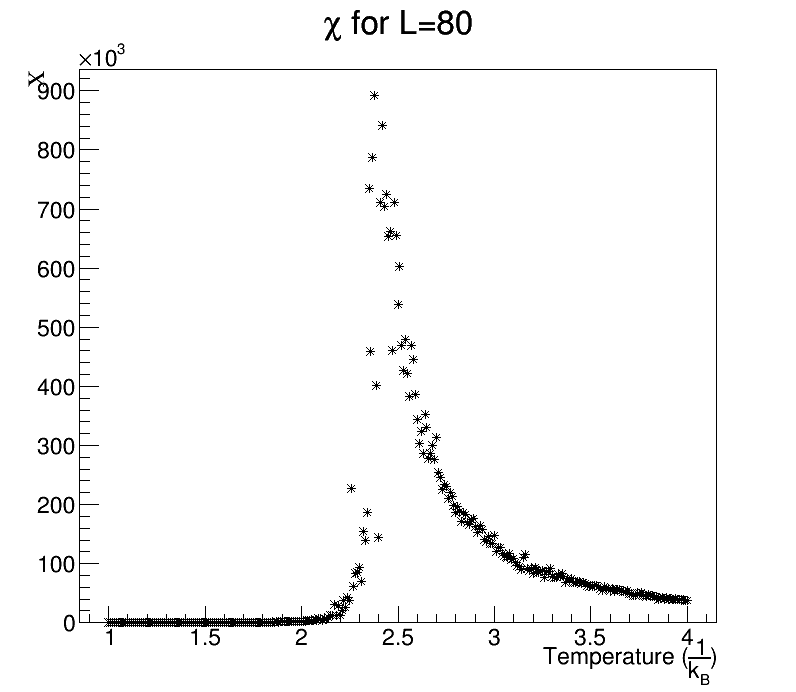
\includegraphics[width=0.27\textwidth]{../Report/plots/parte/susceptibility_latsize80}
}\vspace{-0.4cm}
\caption{Statistical quantities for a $80\times80$ lattice with a steady initial state plotted against the temperature.}
\label{fig:latsize80}
\end{center}
\end{figure}
\end{frame}

\begin{frame}{Estimating $T_{C}\left(L=\infty\right)$}
\begin{itemize}
\item We wish to use these results to determine $T_{C}$ in the limit $L\rightarrow\infty$, using $\nu=1$
\item Accepted value: $T_{C}=2.269/k_{B}$~\cite{lecture}
\item To estimate, we need the information of $T_{C}(L)$. 
\end{itemize} 

\begin{table}[ht]
\begin{center}
\begin{tabular}{c|c|c|c} \hline
L & $T_{C}$ ($1/k_{B}$) (from $C_{V}$) & $T_{C}$ ($1/k_{B}$) (from $\chi$) & Average $T_{C}$ ($1/k_{B}$)\\ \hline
20 & 2.25 & 2.35 & 2.30 \\
40 & 2.30 & 2.35 & 2.33 \\
60 & 2.35 & 2.40 & 2.38 \\
80 & 2.40 & 2.45 & 2.43\\ \hline
\end{tabular}
\caption{Approximate values for $T_{C}(L)$ for $L=20, 40, 60,$ and 80 used with~\eqref{eq:tcscale} to determine $T_{C}(L=\infty)$.}
\label{tab:tcl}
\end{center}
\end{table}
\end{frame}

\begin{frame}{Estimating $T_{C}\left(L=\infty\right)$}
\begin{itemize}
\item We know 
$$
T_{C}(L=\infty)=T_{C}(L)-aL^{-1},
$$
for some $a\in\mathbb{R}$.  So
\begin{align*}
T_{C}(L=\infty) & = \frac{2.30}{k_{B}}-\frac{a}{20} \\
T_{C}(L=\infty) & = \frac{2.33}{k_{B}}-\frac{a}{40} \\
T_{C}(L=\infty) & = \frac{2.38}{k_{B}}-\frac{a}{60} \\
T_{C}(L=\infty) & = \frac{2.43}{k_{B}}-\frac{a}{80}.
\end{align*}
\item Because~\eqref{eq:tcscale} gives us 2 equations in 2 unknowns, and we are looking at four different lattice sizes, we can get any number of 8 possible solutions for $T_{C}$ and $a$.  
\end{itemize}
\end{frame}

\begin{frame}{Estimating $T_{C}\left(L=\infty\right)$}
\begin{itemize}
\item We find $\frac{2.35}{k_{B}}\leq T_{C}\leq\frac{2.575}{k_{B}}$ with error $3.57\%\leq\sigma\leq13.49\%$ compared with the accepted result of $2.269/k_{B}$~\cite{lecture}
\end{itemize}
\end{frame}

\begin{frame}{Estimating $T_{C}\left(L=\infty\right)$}
\begin{figure}[h]
\begin{center}
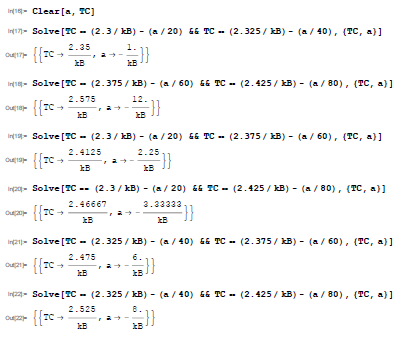
\includegraphics[width=0.7\textwidth]{../Report/solveTC1}
\vspace{-0.4cm}
\caption{Using Mathematica~\cite{mathematica} to solve for the possible values of $T_{C}(L=\infty)$ given the data from Table~\ref{tab:tcl} and~\eqref{eq:tcscale}.}
\label{fig:tcsolve}
\end{center}
\end{figure}
\end{frame}

\section{Testing Random Numer Generators}

\begin{frame}{The Tests}
\begin{itemize}
\item Computer-algorithm random number generators are inherently deterministic, while random number sequences must be uncorrelated.
\begin{itemize}
\item Pseudorandom number generators
\end{itemize}
\item Tests were proposed by Kendall and Babington Smith~\cite{babington} to check whether sequences of numbers were actually random: the frequency, serial, poker, and gap tests.  
\end{itemize}
\end{frame}

\begin{frame}{Frequency Test}
\begin{itemize}
\item Goal: ensure every digit occurs approximately an equal number of times in the sequence~\cite{odell,gruenberger,drueke}.  
\begin{itemize}
\item Distribution is uniform
\item Every digit occurs in the sequence approximately 10\% of the time
\end{itemize}
\end{itemize}
\end{frame}

\begin{frame}{Serial Test}
\begin{itemize}
\item Goal: check no two digits tend to occur in a particular order~\cite{odell,gruenberger,drueke}
\begin{itemize}
\item Like the frequency test, but ensuring all groupings of two digits occur approximately 1\% of the time within the sequence
\end{itemize}
\end{itemize}
\end{frame}

\begin{frame}{Poker Test}
\begin{itemize}
\item Goal: make sure that certain possible combinations of numbers appear with approximately the correct probability.
\item Procedure:
\begin{enumerate}
\item Break digits into blocks of some fixed size (eg. 5 each) 
\item Compare with might be expected in a theoretical poker hand
\end{enumerate}
\item The expected results are shown in Table~\ref{tab:pokeracc}~\cite{drueke} 
\end{itemize}
\begin{table}[ht]
\begin{center}
\begin{tabular}{c|c} \hline
	Hand Type & Frequency (\%) \\ \hline
    5 of a Kind & 0.01\\
    4 of a Kind & 0.45\\
    3 of a Kind & 7.2\\
    2 of a Kind & 50.4\\
    Full House & 0.9\\
    Two Pair & 10.8\\ 
    Other & 30.24\\ \hline
\end{tabular}
\caption{Accepted frequencies for various poker hands~\cite{babington}.}
\label{tab:pokeracc}
\end{center}
\end{table}
\end{frame}

\begin{frame}{$\chi^{2}$ Test}
\begin{itemize}
\item Goal: determine whether there is any correlation between two variables $x$ and $y$.  
\item Procedure:
\begin{enumerate}
\item Compute $\chi^{2}$:
\begin{equation}
\label{eq:chi2}
\chi^{2}=\sum\frac{\left(v-v_{e}\right)^{2}}{v},
\end{equation}
where $v$ is the value observed and $v_{e}$ is the value expected~\cite{babington}  
\item Determine the number of degrees of freedom of the problem, given by 
\begin{equation}
\label{eq:degfree}
DF = (n_{x}-1)*(n_{y}-1),
\end{equation}
where $n_{x}$ is the number of levels of variable $x$ and $n_{y}$ is the number of levels of variable $y$~\cite{chi}. 
\item Consult a $\chi^{2}$ table (or, in our case, an online $p$-value calculator~\cite{graphpad}) to determine the $p$-value given the number of degrees of freedom and the computation of $\chi^{2}$.  We look for $p$ to be above a certain significance level, which we take to be 0.1 (although values of 0.01 and 0.05 are also common)~\cite{drueke}.
\end{enumerate}
\end{itemize}
\end{frame}

\begin{frame}{Degrees of Freedom for $\chi^{2}$ Test}
\begin{table}[ht]
\begin{center}
\begin{tabular}{c|c} \hline
	Test & Degrees of Freedom \\ \hline
     Frequency Test & 9 \\
     Serial Test & 90 \\
     Poker Test & 4 \\ \hline
\end{tabular}
\caption{The degrees of freedom of the various tests used in this analysis~\cite{babington}.}
\label{tab:degfree}
\end{center}
\end{table}
\end{frame}

\begin{frame}{\texttt{ran0}}
\begin{itemize}
\item Minimal Standard Generator -- which is a multiplicative congruential generator~\cite{recipes}
\item Depends on the recurrence relation
\begin{equation}
\label{eq:ran0recur}
I_{j+1}=aI_{j}\mod m
\end{equation}
\item Proposed by Park and Miller with the settings $a=7^{5}=16807$ and $m=2^{31}-1=2147483647$.  
\item Period is expected to be $2^{31}-1=2.1\times10^{9}$~\cite{recipes}.  
\end{itemize}
\end{frame}

\begin{frame}{\texttt{ran0}}
\begin{table}[ht]
\begin{center}
\begin{tabular}{c|c|c} \hline
Statistic & Value & Significance\\\hline
$\mu$ & 4.50159 & 0.04\% \\
$\sigma$ & 2.87309 & 0.45\%\\
$\chi^{2}$ (Frequency Test) & 5.68698 & 0.7708 \\
$\chi^{2}$ (Serial Test) & 86.2657 & 0.5919 \\
$\chi^{2}$ (Poker Test) & 10.0296 & 0.0399 \\ \hline
\end{tabular}
\caption{Results of the frequency, serial, and poker tests performed on \texttt{ran0}, and the significance of those results (the percent difference from the expected value in the case of the mean $\mu$ and the standard deviation $\sigma$, and the $p$-value for the $\chi^{2}$ tests).}
\label{tab:ran0results}
\end{center}
\end{table}
\end{frame}

\begin{frame}{\texttt{ran1}}
\begin{itemize}
\item \texttt{ran1} uses \texttt{ran0} for its random variable but also uses a shuffling algorithm developed by Bays and Durham to remove lower-order correlations:
\begin{itemize}
\item A randomly generated element of the sequence, $I_{j}$, is chosen to be output as some other element of the sequence (typically $I_{j+32}$)
\end{itemize}
\item  Period is expected to be $\sim10^{8}$~\cite{recipes}.
\end{itemize}

\begin{table}[ht]
\begin{center}
\begin{tabular}{c|c|c} \hline
Statsitsic & Value & Significance\\\hline
$\mu$ & 4.50043 & 0.01\%\\
$\sigma$ & 2.87041 & 0.54\%\\
$\chi^{2}$ (Frequency Test) & 7.19849 & 0.6165\\
$\chi^{2}$ (Serial Test) & 112.818 & 0.0522\\
$\chi^{2}$ (Poker Test) & 5.22794 & 0.2647\\ \hline
\end{tabular}
\caption{Results of the frequency, serial, and poker tests performed on \texttt{ran1}, and the significance of those results (the percent difference from the expected value in the case of the mean $\mu$ and the standard deviation $\sigma$, and the $p$-value for the $\chi^{2}$ tests).}
\label{tab:ran1results}
\end{center}
\end{table}
\end{frame}

\begin{frame}{\texttt{ran2}}
\begin{itemize}
\item Claimed to be a "perfect" random number generator (up to floating point errors) by~\cite{recipes}, \texttt{ran2} adds another level of shuffling to further remove the correlations existing in \texttt{ran1}, as well as other randomness checks originally proposed by L'Ecuyer.  
\item Period is expected to be the least common multiple of the periods of the first two algorithms
\begin{itemize}
\item Add the two sequences produced by \texttt{ran0} and \texttt{ran1} modulo the modulus $m$ of either of them ($>10^{8}$)~\cite{recipes}
\end{itemize}
\end{itemize}
\end{frame}

\begin{frame}{\texttt{ran2}}
\begin{table}[ht]
\begin{center}
\begin{tabular}{c|c|c} \hline
Statsitsic & Value & Significance\\\hline
$\mu$ & 4.4999 & $<0.01\%$\\
$\sigma$ & 2.87382 & 0.42\%\\
$\chi^{2}$ (Frequency Test) & 8.62035 & 0.4730\\
$\chi^{2}$ (Serial Test) & 93.7899 & 0.3714\\
$\chi^{2}$ (Poker Test) & 5.28678 & 0.2591\\ \hline
\end{tabular}
\caption{Results of the frequency, serial, and poker tests performed on \texttt{ran2}, and the significance of those results (the percent difference from the expected value in the case of the mean $\mu$ and the standard deviation $\sigma$, and the $p$-value for the $\chi^{2}$ tests).}
\label{tab:ran2results}
\end{center}
\end{table}
\end{frame}

\begin{frame}{\texttt{ran3}}
\begin{itemize}
\item Originally presented by Knuth 
\item Based on subtractive methods -- Fibonacci generator
\begin{itemize}
\item  The next term in the sequence comes from the subtraction of two previous terms. 
\begin{equation}
\label{eq:fibgen}
x_{k}=x_{k-a}-x_{k-b}
\end{equation}
for some fixed $a,b\in\mathbb{Z}$ known as lags.  
\item Fibonacci generators are very efficient and pass most randomness tests thrown at them, although they do require more storage than linear congruential algorithms~\cite{fib} (of which \texttt{ran0}, \texttt{ran1}, and \texttt{ran2} are special cases).
\end{itemize}
\end{itemize}
\end{frame}

\begin{frame}{\texttt{ran3}}
\begin{table}[ht]
\begin{center}
\begin{tabular}{c|c|c} \hline
Statsitsic & Value & Significance\\\hline
$\mu$ & 4.50161 & 0.04\%\\
$\sigma$ & 2.87307 & 0.45\%\\
$\chi^{2}$ (Frequency Test) & 5.92085 & 0.7478\\
$\chi^{2}$ (Serial Test) & 106.29 & 0.1157\\
$\chi^{2}$ (Poker Test) & 7.28835 & 0.1214\\ \hline
\end{tabular}
\caption{Results of the frequency, serial, and poker tests performed on \texttt{ran3}, and the significance of those results (the percent difference from the expected value in the case of the mean $\mu$ and the standard deviation $\sigma$, and the $p$-value for the $\chi^{2}$ tests).}
\label{tab:ran3results}
\end{center}
\end{table}
\end{frame}

\begin{frame}{\texttt{rand()}}
\begin{itemize}
\item Standard in the C++ library
\item Linear congruential algorithm  
\end{itemize}

\begin{table}[ht]
\begin{center}
\begin{tabular}{c|c|c} \hline
Statistic & Value & Significance\\\hline
$\mu$ & 4.50236 & 0.05\%\\
$\sigma$ & 2.87138 & 0.51\%\\
$\chi^{2}$ (Frequency Test) & 7.25112 & 0.6110 \\
$\chi^{2}$ (Serial Test) & 79.4787 & 0.7784 \\
$\chi^{2}$ (Poker Test) & 3.55947 & 0.4689 \\ \hline
\end{tabular}
\caption{Results of the frequency, serial, poker, and gap tests performed on \texttt{ran4}, and the significance of those results (the percent difference from the expected value in the case of the mean $\mu$ and the standard deviation $\sigma$, and the $p$-value for the $\chi^{2}$ tests).}
\label{tab:ran4results}
\end{center}
\end{table}
\end{frame}

\begin{frame}{Effect on Physics}
\begin{itemize}
\item Overall, we find that the choice of random number generator didn't have major contributions to the results determined.  However, small differences were observed.\footnote{Throughout this discussion, we are working with the generation of a $2\times2$ lattice with an initial random configuration at a temperature of $T=1/k_{B}$.} 
\begin{itemize}
\item Example, it was observed that, if we plotted the number of accepted MC against the total number of MC cycles used in the calculation, the slopes were slightly different.   In particular, \texttt{ran1}, \texttt{ran3}, and \texttt{rand()} have more accepted MC than do \texttt{ran0} or \texttt{ran2}.  
\end{itemize}
\end{itemize}
\end{frame}

\begin{frame}{Effect on $\chi$}
\vspace{-0.4cm}
\begin{figure}[h]
\begin{center}
\subfigure[]{
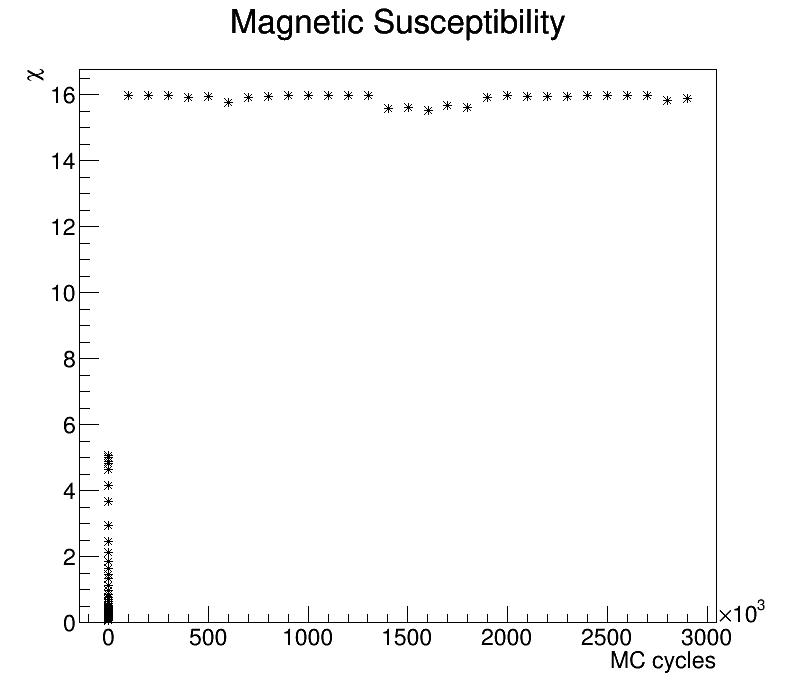
\includegraphics[width=0.27\textwidth]{../Report/benchmarks/ran0/plots_random_chi_size2_temp1}
}
\subfigure[]{
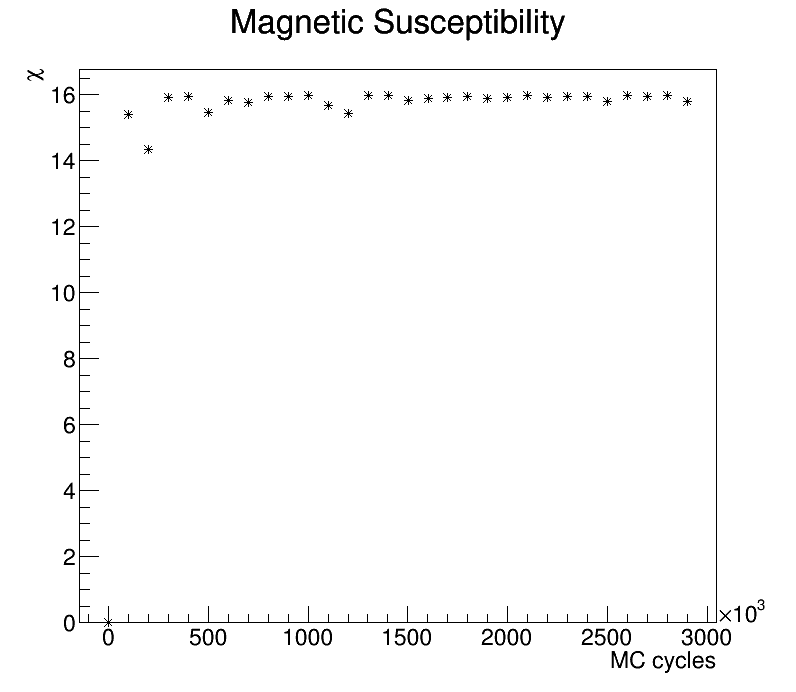
\includegraphics[width=0.27\textwidth]{../Report/benchmarks/ran1/plots_random_chi_size2_temp1}
} 
\subfigure[]{
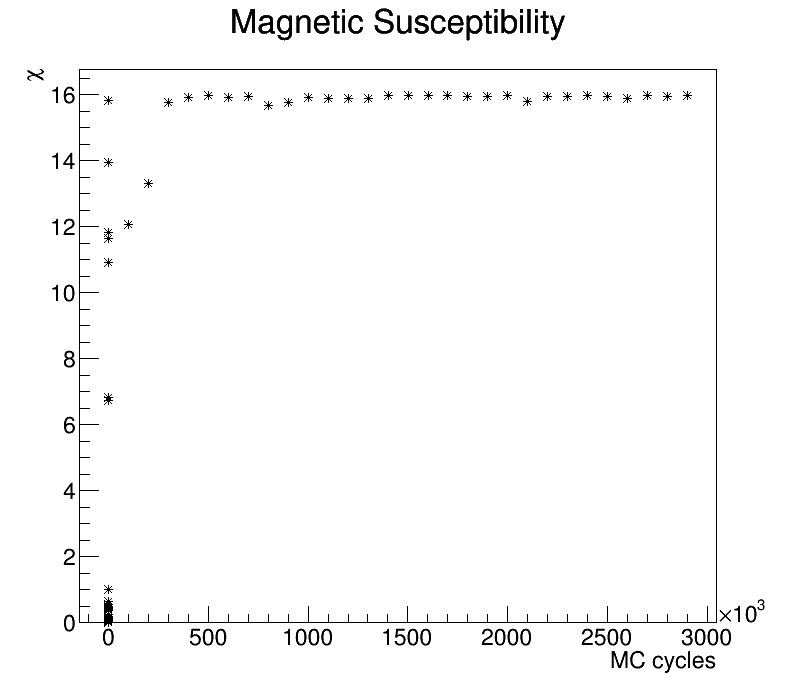
\includegraphics[width=0.27\textwidth]{../Report/benchmarks/ran2/plots_random_chi_size2_temp1}
}\\ \vspace{-0.3cm}
\subfigure[]{
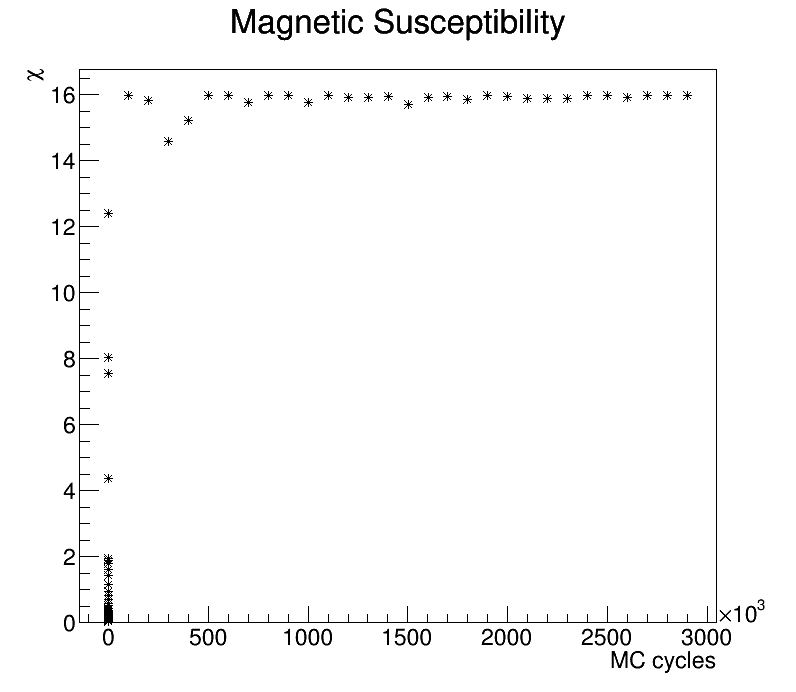
\includegraphics[width=0.27\textwidth]{../Report/benchmarks/ran3/plots_random_chi_size2_temp1}
} 
\subfigure[]{
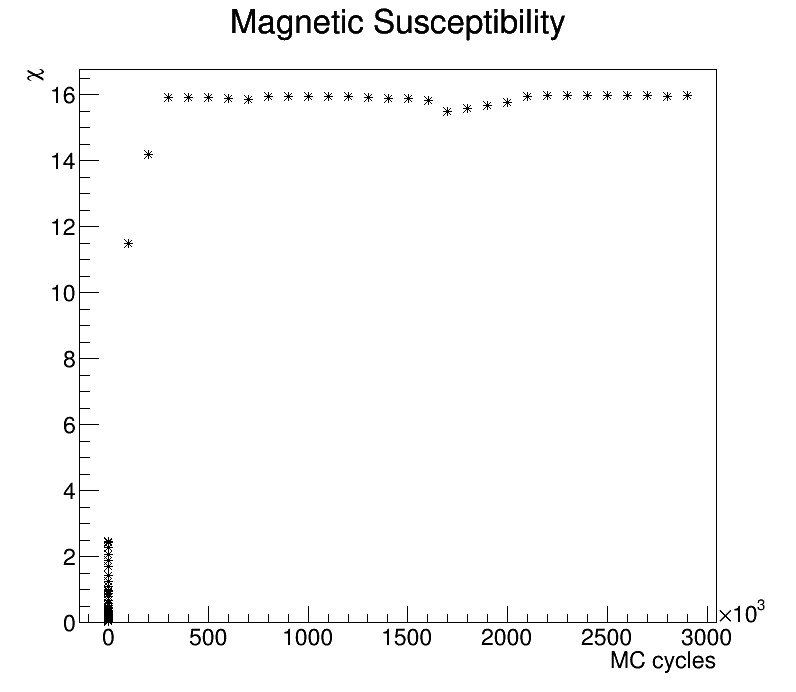
\includegraphics[width=0.27\textwidth]{../Report/benchmarks/plots/plots_random_chi_size2_temp1}
}\vspace{-0.4cm}
\caption{Magnetic susceptibility $\chi$ as a function of the number of MC cycles used in the calculation for (a) \texttt{ran0}, (b) \texttt{ran1}, (c) \texttt{ran2}, (d) \texttt{ran3}, and (e) \texttt{rand()}.}
\label{fig:randoschi}
\end{center}
\end{figure}
\end{frame}

\section{Conclusions}

\begin{frame}{Conclusions}
\begin{itemize}
\item Developed framework for implementation of Ising model in two dimensions
\item Used framework to calculate and analyze various statistical quantities
\item Used statistical quantities to estimate $T_{C}$ for an infinite lattice to within $14\%$ of the accepted value
\item Tested various random number generators for randomness and effect on physics
\end{itemize}
\end{frame}

\begin{frame}{Thank you!}
Thank you to Morten Hjorth-Jensen for all of his help throughout this semester with this and the other projects.
\\Thank you to John Hall for allowing me to include the pseudorandom sequence in this analysis.
\\Thank you to Christie Campbell whose slide formatting I used for this presentation.
\end{frame}

\begin{frame}{Questions}
\begin{figure}[h]
\begin{center}

\includegraphics[width=0.7\textwidth]{Graduation}
\end{center}
\end{figure}
\end{frame}

\bibliographystyle{abbrv}
\bibliography{mybib}

\end{document}